% =====================================================================
% LaTeX Template for the International Journal of Disaster Risk Reduction
% Author: Alexandre Dunant
% Based on Elsevier's elsarticle class
% =====================================================================

\documentclass[preprint,12pt,authoryear]{elsarticle}

% -------------------- PACKAGES --------------------
\usepackage[utf8]{inputenc}
\usepackage[T1]{fontenc}
\usepackage{lmodern}
\usepackage{amsmath,amssymb}
\usepackage{graphicx}
\usepackage{booktabs}
\usepackage{caption}
\usepackage{subcaption}
\usepackage{url}
\usepackage{hyperref}
\usepackage{lineno}
\usepackage{xcolor}
\usepackage{float}

% -------------------- SETTINGS --------------------
\linenumbers                    % Enable line numbers for review
\journal{International Journal of Disaster Risk Reduction}

% Hyperref setup
\hypersetup{
    colorlinks=true,
    linkcolor=blue,
    citecolor=blue,
    urlcolor=blue,
    pdftitle={Multi-hazard scenario ensembles for estimating earthquake risk},
    pdfauthor={Alexandre Dunant}
}

% Bibliography style: author-year
\bibliographystyle{elsarticle-harv}

% -------------------- DOCUMENT --------------------
\begin{document}

\begin{frontmatter}

\title{Multi-hazard scenario ensembles for estimating earthquake risk}

\author[inst1,inst2]{Alexandre Dunant\corref{cor1}}
\author[inst3]{Tom R. Robinson}
\author[inst1]{Alexander L. Densmore}
\author[inst4]{Sweata Sijapati}
\author[inst1]{Nick J. Rosser}
\author[inst5]{Mark Kincey}
\author[inst6]{Katie J. Oven}

% Use \cortext for the corresponding author details
\cortext[cor1]{Corresponding author; now at EURAC, Bolzano, Italy. Email: Alexandre.dunant@eurac.edu}

% Define the addresses using the [instX] labels
\address[inst1]{Institute of Hazard, Risk, and Resilience and Department of Geography, Durham University, Durham, UK}
\address[inst2]{Center for Climate Change and Transformation, EURAC, Bolzano, Italy}
\address[inst3]{School of Earth and Environment, University of Canterbury, Christchurch, New Zealand}
\address[inst4]{National Society for Earthquake Technology, Kathmandu, Nepal}
\address[inst5]{School of Geography, Politics, and Sociology, Newcastle University, Newcastle, UK}
\address[inst6]{Department of Geography and Environmental Sciences, Northumbria University, Newcastle, UK}

\begin{abstract}
Building on previous shaking-only scenario approaches, this study incorporates cascading hazards—earthquake-triggered landslides—using a hypergraph network model to efficiently quantify risk in cascading multi-hazard scenario ensembles. We apply this model to an ensemble of 30 plausible large-magnitude earthquakes ($M_w > 7$) across Nepal to evaluate the combined impacts of shaking and landsliding on building and road infrastructure. While shaking damage dominates the overall impact profile, our findings reveal that landslides substantially increase the spatial extent of risk, particularly in steep and remote regions where landslide impacts can exceed $\text{50\%}$ of shaking-related damage. The results demonstrate a significant correlation between district remoteness and vulnerability to road damage, creating compounding challenges for emergency response and healthcare access. These findings highlight an urban-rural risk divide shaped by Nepal's diverse topography. This multi-hazard ensemble approach provides a more comprehensive understanding of earthquake risk than shaking-only assessments, offering valuable insights for contingency planning by humanitarian organizations and the Government of Nepal.
\end{abstract}

\begin{keyword}
cascading multi-hazards \sep multi-hazard modelling \sep earthquake scenarios \sep earthquake impacts \sep landslides \sep Nepal \sep network modelling
\end{keyword}

\end{frontmatter}

% -------------------- MAIN TEXT --------------------

\section{Introduction}
Earthquakes have killed more than two million people since 1900 \citep{England2011,Daniell2017} and remain one of the deadliest global hazards. Humanitarian contingency planning for future earthquakes -- which comprises both preparation for earthquake response as well as pre-emptive efforts to reduce the impacts from a future earthquake \citep{IASC2007,IFRC2012} -- is most likely to be effective if it is based on the best available scientific information on the associated risks \citep{Alexander2007}. This information should ideally include estimates of the scale of impacts in a future earthquake as well as the locations where impacts are most likely to occur \citep{IASC2007}.

In contingency planning, the emphasis is typically placed exclusively on worst-case or maximum credible events. It can be useful, however, to distinguish between a range of possible or plausible impacts, especially when planning involves the allocation of often scarce resources. Existing approaches to seismic risk analysis typically fall into one of two categories \citep{Robinson2018}. Deterministic approaches use scenarios that define the effects of one or a small number of possible future earthquakes \citep{Davies2015}, often chosen as the `maximum credible event' or the worst-case event that could be expected on a particular fault. In contrast, probabilistic approaches rely on estimates of the likelihood of exceeding a given value of ground motion from all possible seismic sources over a specified period of time, with the corresponding impacts from that level of shaking representing the total cumulative losses over the time period.

Building upon a body of work that has critically reviewed both probabilistic and deterministic approaches \citep{Bommer2002,Wang2003,Wang2011,Bilham2013}, Robinson et al. \citep{Robinson2018} noted that, for many of the world's earthquake-prone areas, there are insufficient data on past earthquakes and their impacts to reliably apply either method. Borrowing from common practice in climate modelling, they proposed an alternative approach that used an ensemble of earthquake scenarios to identify patterns of emergent impacts. This allowed them to distinguish between consequences that were common to multiple scenarios -- and thus more likely to occur in future -- from those that were highly specific to a single future event \citep{Robinson2018}. They applied this ensemble approach to evaluate relative earthquake risk in Nepal to support contingency planning by the Humanitarian Country Team in Nepal. Importantly, because the different scenarios were equally weighted in the ensemble, they focused exclusively on relative risk between scenario outcomes.

An important shortcoming of the scenario ensemble developed by Robinson et al. \citep{Robinson2018}, however, is that it only considered damage to buildings resulting from earthquake shaking. Experience in recent large continental earthquakes shows that shaking damage is only one part of a common chain of earthquake-related hazards \citep{Gill2014}. Landslides, debris flows, sediment aggradation, and subsequent flooding can have persistent impacts for years or decades after the earthquake \citep{Fan2019,Kincey2021}, and earthquakes that trigger landslides typically have larger impacts than those that do not \citep{Budimir2014}. Planning for future earthquake impacts in continental settings should therefore account for this range of earthquake-related hazards.

Promisingly, multi-hazard approaches to risk assessment are now becoming more widespread (see recent reviews by \cite{Gill2022,Ward2022}). Multi-hazards are defined by UNDRR (\url{https://www.undrr.org/terminology/hazard}) as "events may occur simultaneously, cascadingly or cumulatively over time, and taking into account the potential interrelated effects". While many "multi-hazard" risk models overlay single hazards without considering their interactions \citep{Gill2014}, there is growing recognition that true multi-hazard risk assessment requires models that can consider interactions between different hazards and can capture spatial clustering or amplification effects \citep{Mignan2014,Tilloy2019,Dunant2021,Ming2022,Hochrainer-Stigler2023}.

Dunant et al. \citep{Dunant2025} proposed a novel multi-hazard impact model that used a hypergraph framework to link elements at risk -- such as buildings or roads -- within spatial domains corresponding to the areas exposed to a hazard trigger such as an earthquake. The hypergraph approach allowed efficient estimation of the impacts from cascading multi-hazards; in turn, this efficiency meant that the impacts of a scenario earthquake could be simulated repeatedly within a Monte Carlo framework to derive statistical estimations of the areas most likely to be affected. They evaluated the model against the 2015 Mw 7.8 Gorkha earthquake in Nepal, and showed that the model could reasonably approximate the spatial patterns of building damage due to shaking as well as building and road damage due to earthquake-triggered landslides.

Here, we apply the multi-hazard impact model of Dunant et al. \citep{Dunant2025} to the scenario ensemble analysed by Robinson et al. \citep{Robinson2018}, in order to provide the first quantitative estimates of a suite of potential multi-hazard impacts arising from the next earthquake to occur in Nepal. This provides a substantially more complete picture of both the number and spatial distribution of earthquake-related impacts, including those arising from cascading hazards such as earthquake-triggered landslides, than was previously possible. Our purpose is not to predict the specific details of a future earthquake. Instead, we aim to illustrate the range of potential impacts that could arise from a suite of plausible earthquake scenarios, and the areas most likely to be affected by earthquake shaking and earthquake-triggered landslides, in order to support contingency planning for a future event by the Humanitarian Country Team and the Government of Nepal \citep{Sijapati2024}.

\section{Methods}
We first provide a brief description of the hypergraph multi-hazard impact model. We then describe the earthquake scenario ensemble that we use to drive the model, and the experimental setup.

\subsection{Model description}

A full description of the hyperedge multi-hazard impact model was provided by Dunant et al. \citep{Dunant2025}, along with details of its application to the 2015 Mw 7.8 Gorkha earthquake. Here, we give an overview of the model and its key assumptions. The model operates on a network of nodes which represent the elements in the model -- in this case, hillslopes (represented by individual slope units), buildings, and roads. These nodes are connected by hyperedges, which can be thought of as polygons that enclose one or more nodes. Unlike edges in graph-based models which link a single pair of nodes \citep{Dunant2021}, hyperedges can connect multiple nodes. For example, in the model used here a single hyperedge links all slope units within Nepal. Those slope units, in turn, can be represented by individual hyperedges that link all of the buildings and roads on each hillslope. In this way, we can define a nested set of hyperedges that preserve both the characteristics of each element -- for example, the topography of each slope unit, or the building type, or the susceptibilities to landslides or debris flows at each building location -- and the spatial relationships between those elements. The efficiency of the hypergraph network means that hundreds or thousands of separate simulations can be run for each earthquake scenario, with each simulation exploring a different pathway through the network of possible cascading impacts \citep{Dunant2025}. A Monte Carlo approach allows us to quantify uncertainty within a single scenario by generating a statistical distribution of possible outcomes \citep{Dunant2021}. By applying this process to each earthquake in an ensemble of plausible scenarios, we also capture inter-scenario variability. In this way, we combine two distinct sources of uncertainty: the variability in how impacts may propagate from a single earthquake, and the variability in impacts across different possible earthquakes. This allows us to derive both per-scenario uncertainty and relative probabilistic outputs for the ensemble as a whole.

The implementation of the model described here is focused on the chain of hazards associated with large continental earthquakes. Earthquake shaking is assumed to cause direct damage to buildings via a set of fragility functions that relate peak ground acceleration (PGA) to the probability of reducing the building to a complete damage state (Figure S1). Shaking can also trigger landslides within individual slope units that fall within the footprint of the earthquake, and those landslides in turn may damage buildings or road segments within the slope unit. Because our focus is on the direct impacts of our chosen scenario earthquakes, we do not consider longer term or delayed hazards such as landslide reactivation by subsequent rainfall \citep{Fan2019,Kincey2021}, or consequent downslope changes in sediment storage and flood capacity. Thus, our results should be interpreted as reflecting the instantaneous coseismic effects that could be observed on the day of the earthquake. Other hazards, such as those triggered directly by rainfall, are also not considered, although they could be added via additional sets of hyperedges and interactions.

To generate a single earthquake impact scenario, we apply the expected ground shaking from our chosen earthquake to the hyperedge model and evaluate 10,000 separate outcomes from that event -- that is, we repeat the hyperedge model 10,000 times, each time following a separate path through the hyperedge network. This generates a distribution of model outcomes in terms of the likelihood that any building will be damaged by earthquake shaking or by landsliding, and the likelihood that any 100 m road segment will be damaged by landsliding. Those likelihoods can then be aggregated by administrative unit to identify the areas most likely to be affected by one or another of those components in the earthquake hazard chain. We then repeat this process for the other scenario earthquakes, and examine the ensemble of outcomes that result.

\subsection{Earthquake ensemble}

Robinson et al. \citep{Robinson2018} adopted an ensemble of 30 large ($M_w > 7$) earthquakes that could plausibly cause damage in Nepal, based on a combination of historical records and palaeoseismic evidence along with the distribution of major faults (Figure~\ref{fig:study}). These included earthquakes along the Main Himalayan Thrust, ranging in magnitude from $M_w$ 7.3 to 8.6, as well as earthquakes in the upper plate of the Main Himalayan Detachment on the Karakorum Fault ($M_w$ 7.8), the northern ($M_w$ 7.8) and southern ($M_w$ 7.3) parts of the Western Fault System, and the Thakkhola Graben ($M_w$ 7.3). For direct comparison of our modelling with their results, we adopt the same 30 scenario earthquakes. We model the pattern of PGA for each of these 30 events with OpenSHA \citep{Field2003}, using the ground motion prediction equations of Abrahamson and Silva \citep{Abrahamson2008}, exceedance probabilities of $\text{50\%}$, and shallow shear wave velocity (Vs30) derived from topographic slope \citep{Allen2009}. Maps of PGA for each of the 30 scenario earthquakes are shown in Figure S2.

\begin{figure}[H]
    \centering
    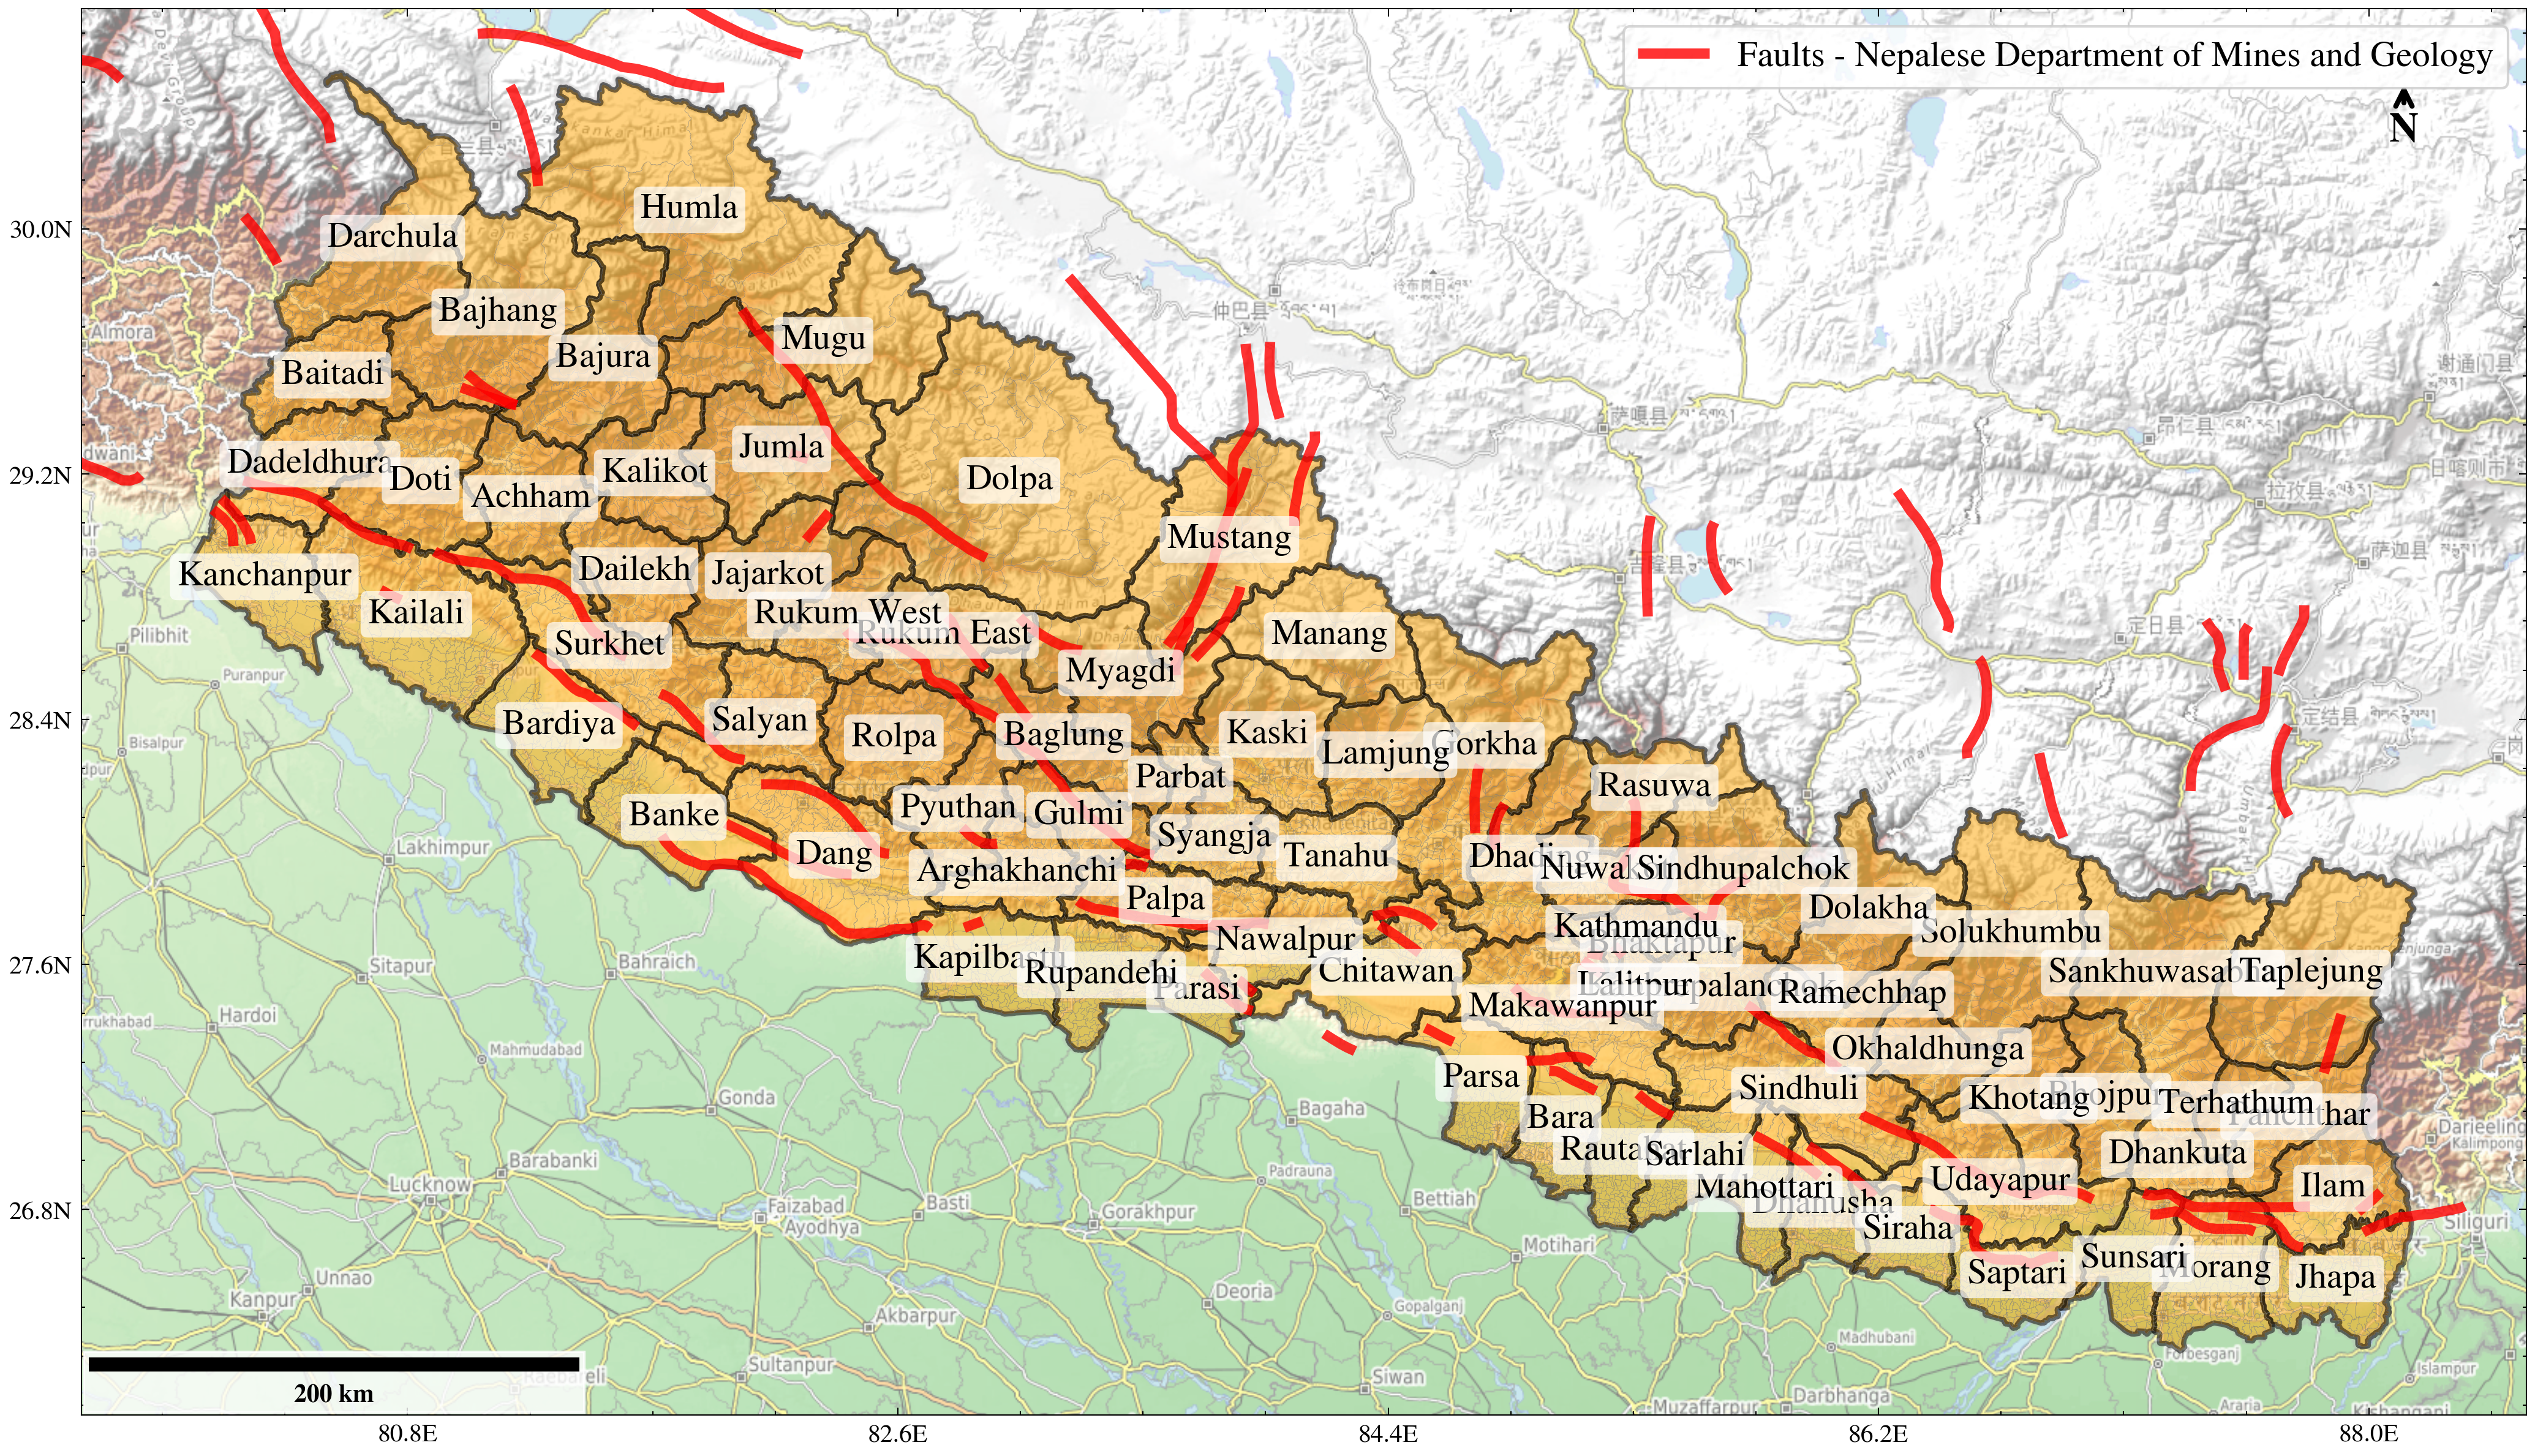
\includegraphics[width=1\linewidth]{./FIGURES/Fig1_study_area_map.png}
    \caption{Map of districts and major fault systems in Nepal.}
    \label{fig:study}
\end{figure}


\section{Experimental setup and data sources}

For each scenario earthquake, the model proceeds through the hyperedges that connect earthquake shaking to other elements in the model, checking to see whether each hyperedge is activated -- that is, whether a building is damaged by shaking or a slope unit is affected by one or more landslides. If that hyperedge is activated, then the simulation propagates along that hyperedge and can cascade to other hyperedges through the network.

We first check the buildings within the footprint of the earthquake (defined by a PGA cutoff value of $0.1\,\text{g}$, below which the probability of complete damage is low for all building types; see Figure S1). We use building locations taken from the Humanitarian OpenStreetMap Team available from \url{https://data.humdata.org/dataset/hotosm_npl_buildings}, comprising approximately 7.1 million building polygons. Construction types are not available for individual building polygons, so we use the best-available national-scale exposure data from the Modelling Exposure Through Earth Observation Routines (METEOR) project, available from \url{https://maps.meteor-project.org/map/building-exposure-map-of-nepal}. This dataset provides the relative proportions of different building types within each $90 \times 90\,\text{m}$ grid cell. For each building type, we define three separate fragility functions -- a `Low', `Mid', and `High' case -- representing the uncertainty in its structural performance (Figure S1). We then generate a single, representative fragility function for each grid cell by calculating a weighted average of these functions, where the weights are determined by the proportions of each building type in that cell. We then compare the weighted-average fragility function in each cell to the PGA value at the cell centroid to determine the likelihood of complete damage for each building $[0,1]$ for the low-, mid- and high-fragility cases. Dunant et al. \citep{Dunant2025} showed that the mid-fragility case was best able to reproduce observed building damage patterns and numbers in the 2015 Gorkha earthquake, so for simplicity we focus on the results with the mid-fragility case below.

For each slope unit, we compute the mean PGA value and use it to determine the probability of landsliding based on a lognormal function that is calibrated by observations in the 2015 Gorkha earthquake \citep{Dunant2025}. We then compare this probability against a uniform random deviate to decide whether a slope unit is `activated' during a simulation. Over multiple simulations, slopes that were more likely to slide will be activated more frequently. However, due to the probabilistic nature of this approach, the exact pattern of activations can vary between simulations. For each slope unit that is activated, the model proceeds to determine whether landslides are triggered and, if so, whether they impact buildings or road segments within that unit. To do so, we evaluate landslide susceptibility using a model that relies exclusively on topographic variables (i.e. no earthquake related information). This model incorporates seven key factors: elevation, hillslope aspect, proximity to rivers, plan-view curvature, regional relief, local slope gradient, and a terrain ruggedness index. These factors are derived from a $10\,\text{m}$ resolution digital elevation model (DEM), which was created by downsampling the $5\,\text{m}$ DEM provided by the Advanced Land Observing Satellite World 3D (\url{https://www.aw3d.jp/en/products/standard/}). We applied the XGBoost machine learning algorithm, implemented in Python, to develop the susceptibility model. For the purposes of this study, the model was trained using data from coseismic landslides triggered by the 2015 Gorkha earthquake, as documented by Kincey et al. \citep{Kincey2021}. The model achieved an area under the receiver operating characteristic (ROC) curve of $0.75$. It should be emphasized that this susceptibility model is optimized for the 2015 Gorkha earthquake, and it is possible to use other susceptibility models within the hyperedge framework as required.

Whether or not a landslide is triggered in the slope unit is determined by drawing a value from a Gaussian distribution of landslide susceptibility with the same mean and standard deviation as the distribution of susceptibility values in that slope unit, and comparing that value with a uniform random deviate \citep{Dunant2025}. If the susceptibility value is smaller than the random deviate, then no landslide occurs and propagation along that hyperedge stops. If a landslide is triggered in a given slope unit, we perform a secondary check to assess whether individual buildings and road segments within that unit are impacted. This is done by comparing the landslide susceptibility value at the location of each asset (representing potential impact probability) with a uniform random deviate. If the deviate exceeds the susceptibility value, the asset is considered unaffected; otherwise, we assume it is impacted by the landslide and track the event. While the slope-unit-scale susceptibility governs the triggering of landslides, the local susceptibility value at each asset location is used as a proxy for spatially-variable impact likelihood. Because the susceptibility model is trained on the full footprint of coseismic landslides \citep{Kincey2021}, this impact likelihood encompasses both source and runout areas. This process is repeated iteratively across all activated slope units to generate a cascading impact scenario, simulating the spread of landslides and their effects on infrastructure throughout the region. We continue this process iteratively to search through all slope units in the network to generate a single outcome for that earthquake. This is repeated 10,000 times for each scenario earthquake. This results in a shaking impact likelihood and a landslide impact likelihood, both in the range $[0,1]$, for each building, and a landslide impact likelihood in the range $[0,1]$ for each $100\,\text{m}$ road segment in our national-scale dataset. Finally, we move on to the next earthquake in the 30-member ensemble and repeat the steps above.

\section{Analysis of ensemble outcomes}

Robinson et al. \citep{Robinson2018} focused on scenario earthquake impacts in terms of fatalities, using statistical relationships between building damage states, building occupation rates, and fatality rates. Because occupation rates vary over time (e.g., between day and night), they also considered three possible occurrence times for each of the 30 scenario earthquakes. Here, we focus instead on earthquake impacts on (static) buildings and roads, both through shaking and earthquake-triggered landsliding, and so we limit our analysis to the 30 earthquakes without considering occurrence time. Extending our multi-hazard results to estimate fatalities would require well-established empirical functions to relate landslide occurrence to fatality rates for people in buildings and using the road network \citep{VanWykDeVries2024}. These do not yet exist, although there is some recent research toward that goal \citep{Pollock2020,Luo2023,Hu2024}. Our choice to focus on the impacts to infrastructure is justified also by the common need in humanitarian contingency planning to focus on the numbers of affected households who will potentially require assistance \citep{IASC2007}. The detailed relationship between the locations of infrastructure, which are typically known, and the locations of people in the landscape over time, which are typically not known, remains an outstanding gap, and we return to this point in the discussion.

While the hypergraph model generates an impact likelihood for each building and each $100\,\text{m}$ road segment in our infrastructure database, it is important to remember that this is only valid in a probabilistic sense and does not represent a statement that `building X will be damaged in earthquake N'. Dunant et al. \citep{Dunant2025} showed that the performance of the hypergraph model in the 2015 Gorkha earthquake, in terms of its ability to reproduce observed patterns of damage, improved as the model results were aggregated over larger and larger administrative areas. They identified the district level ($n = 77$ in Nepal) as providing the optimum trade-off between model performance and granularity of results. Despite not featuring in Nepal's federal structure after the adoption of the new constitution in 2015, district governments remain important for disaster management \citep{Bhandari2020}. Accordingly, we primarily aggregate our results at district level in the sections below. We do this by calculating the expected value of (1) buildings damaged by earthquake shaking, (2) buildings damaged by either earthquake shaking or landsliding, and (3) road segments damaged by landsliding, taking each as the sum of the per-building (or per road segment) likelihood values in that district. For example, if a district contains 10 buildings and the mean per-building likelihood of damage by shaking is $0.5$, then on average we would expect 5 buildings to be completely damaged in any given earthquake. This approach assumes that the likelihood of damage is independent between buildings and between road segments, and is not spatially correlated (e.g., through co-location on a large landslide mass).

We use the expected numbers of buildings damaged by shaking, buildings damaged by shaking or landsliding, and road segments damaged by landsliding to estimate the exceedance probability of impacts across the 30 scenario earthquakes. This allows us to determine both the median and worst-case for each type of impact and within each of Nepal's 77 districts.

We also examine the variability of each of our three types of impact across the different scenarios. If all scenarios result in similar impacts within a district, then the potential impacts are likely to occur irrespective of the details of the next earthquake. Conversely, if the impacts vary greatly between the different scenarios, then there is high uncertainty about what could occur in the next event. To capture this, we calculate the standard deviation of damage across the 30 ensemble members for each district. High standard deviation indicates that damage is highly dependent on the specific earthquake scenario, whereas low standard deviation suggests a more consistent risk profile regardless of the specific event.

\section{Multi-Hazard Risk Scores}

To move beyond single-hazard assessments and identify districts where risk is specifically related to one hazard type or where different risks compound, we developed two multi-hazard risk scores. These scores are driven by an ensemble of 30 plausible, large-magnitude earthquake scenarios to capture a range of potential outcomes. Both scores incorporate a remoteness factor, which serves as a proxy for the logistical challenges of post-disaster aid delivery. This factor, based on feedbacks from the Humanitarian Country Team in Nepal and the work presented in \cite{Robinson2018}, measures accessibility by considering distance from roads, key services, and transportation methods. As an example, Districts with high remoteness scores will likely be slower to receive aid after a large earthquake.

We use remoteness index values estimated by \cite{banick2019}, who quantified physical remoteness using a geographic information system-based cost-time model that calculated travel times from any location to essential services. They integrated digital elevation data, road networks, land cover, and seasonal conditions to model realistic travel impedance across varied terrain, using a $30\,\text{m}$ resolution raster grid across all of Nepal. Their model accounted for topographic constraints by implementing switchback algorithms for steep slopes, assigned different speeds to four hierarchical road classes, and incorporated seven land cover categories for off-road travel. Seasonal accessibility variations were captured through separate dry and monsoon season models, with appropriate speed reductions applied to different road types during adverse conditions. The resulting travel time estimates were validated by \cite{banick2019} against household survey data and expert consultations, then aggregated by administrative units to produce separate remoteness metrics for dry and monsoon seasons. Their results specify the fraction of the population in each administrative unit for whom essential services can be accessed within one of eight time intervals ($0$--$30$ minutes, $30$ minutes--$1$ hour, $1$--$2$ hours, $2$--$4$ hours, $4$--$8$ hours, $8$--$16$ hours, $16$--$32$ hours, and $>32$ hours).

For our analysis, we focus on travel time to two different types infrastructures: district headquarters, representing access to government support, and health facilities, both essential facilities in disaster response \citep{NationalPlanningCommission2015}. We weight the travel time intervals with a progressive weighting scale where weights increase exponentially with travel time, ranging from $0.05$ for areas within 30 minutes of facilities to $2.5$ for areas more than 32 hours away. These weights are then multiplied by the percentage of population in each travel time interval to calculate a weighted remoteness value for each district. This weighting approach ensures that districts with larger populations facing longer travel times receive appropriately higher remoteness scores. So, for each district, the remoteness index $\text{RI}$ for either access to district headquarters or health facilities is calculated as:

\begin{equation}
\label{eq:remoteness-index}
\text{RI} = \sum_{i} \left( w_{i} \times P_{i} \right)
\end{equation}

where $w_{i}$ represents the weight for travel time interval $i$, and $P_{i}$ represents the fraction of the district's population falling within that travel time interval. The resulting indices are normalised to a $0$--$1$ scale by dividing by the highest district value.

To objectively categorise districts by remoteness level, we employ a data-driven statistical approach rather than arbitrary thresholds. We use K-means clustering with silhouette analysis to determine the optimal number of remoteness categories. The silhouette score, which measures how well-defined and separated the clusters are, is calculated for cluster numbers ranging from 2 to 10 (Figure S4). The number of clusters yielding the highest silhouette score is selected as optimal for our dataset. We obtain three groups corresponding to low, medium, and high remoteness. Finally, risk scores are calculated by multiplying worst-case impact values (buildings and roads damaged) by the corresponding remoteness indices and summing the result at the administrative scale of interest.

We define the following variables for use in the risk score formulas:
  \begin{itemize}
      \item $R$: The remoteness index
      \item $S$: The worst-case shaking damage (absolute or proportional).
      \item $L$: The worst-case landslide damage (absolute or proportional).
  \end{itemize}

\subsection{Absolute Compounding Risk Score}

This index is designed to identify hotspots of large-scale, compounding disaster, which is particularly useful for humanitarian contingency planning. The score combines remoteness with absolute worst-case damage using a weighted sum approach. The formula is:

\begin{equation}
\label{eq:absolute-risk-score}
\text{Risk Score}_{\text{Absolute}} = 0.5 \times R + 0.5 \times \frac{S + L}{\max(S + L)}
\end{equation}

where $R$ is the normalized remoteness index, $S$ is the absolute worst-case shaking damage (number of buildings), and $L$ is the absolute worst-case landslide damage (number of buildings and road segments combined). The total impact $(S + L)$ is normalized before being combined with remoteness in a weighted sum. This approach treats remoteness and disaster magnitude as two independent but equally important components (50\% weight each). Districts score high if they have either high remoteness or high total impact, or both. This score helps identify areas requiring substantial humanitarian response.

\subsection{Normalized Risk Score}

This index identifies districts where the community is most severely threatened, regardless of its size. It combines remoteness with proportional worst-case damage. The calculation is:

\begin{equation}
\text{Risk Score}_{\text{Normalized}} = 0.5 \times R + 0.25 \times \frac{S_{\text{prop}}}{\max(S_{\text{prop}})} + 0.25 \times \frac{L_{\text{prop}}}{\max(L_{\text{prop}})}
\end{equation}

where $R$ is the normalized remoteness index, $S_{\text{prop}}$ is the proportional worst-case shaking damage (percentage of buildings), and $L_{\text{prop}}$ is the proportional worst-case landslide damage (percentage of buildings and road segments). Each hazard type is normalized independently before being combined. This weighted sum approach (50\% remoteness, 25\% shaking, 25\% landslides) highlights small, remote districts that lose high percentages of their infrastructure.

The spatial distribution of these risk scores across Nepal is illustrated in Figure~\ref{fig:risk_score}.

\section{Results}

\subsection{Multi-hazard impacts}

The total modelled number of buildings damaged by shaking varies between the different earthquakes in the ensemble, from approximately 8,600 for a Mw 7.8 Karakoram earthquake to approximately 3,400,000 for a Mw 8.6 in the Midwest, West, and Central regions of Nepal. For comparison, the Mw 7.8 Gorkha earthquake in central Nepal caused the destruction or damage of 981,000 buildings \citep{NationalPlanningCommission2015}. In contrast, the number of modelled building impacts by landsliding varies from approximately 80 for the Karakorum earthquake to approximately 178,000 for the same Mw 8.6 event, and the number of modelled 100 m road segments impacted by landsliding varies from just over 100 to approximately 150,000 for the same earthquakes. Total landslide impacts are thus smaller than shaking impacts by 1--2 orders of magnitude for any given earthquake within the ensemble.

Exceedance probability curves (Figure~\ref{fig:exceedance}) indicated that median national-level impacts include approximately 600,000 buildings damaged by shaking, 32,000 buildings damaged by landslides, and 29,000 road segments damaged by landslides. These distributions are right-skewed, with fewer high-damage scenarios reflecting the fact that large impacts occur in only a subset of the modelled events.

\begin{figure}[H]
    \centering
    \includegraphics[width=1\linewidth]{./FIGURES/Fig2_exceedance_probability.png}
    \caption{Exceedance probability of buildings damaged by earthquake shaking (grey), buildings damaged by landslides (light blue), and road segments damaged by landslides (medium blue) across the 30 scenario earthquakes.}
    \label{fig:exceedance}
\end{figure}

The number of modelled earthquake impacts, and thus the ratio of damage by landslides to damage by shaking, varies strongly across Nepal, depending upon both the shaking patterns in the scenario earthquakes and the underlying susceptibility to landsliding. Thus, while building damage from earthquake shaking represents the largest single category of damage in all of Nepal’s 77 districts, its proportion of the total number of impacts is highly variable (Figure~\ref{fig:district_ratio}). If we consider the worst-case event for each district, landslide impacts on buildings and roads make up between 1\% and 84\% of the number of buildings damaged by shaking. The ratio is lowest for districts located in the low-elevation, low-relief Terai region in southern Nepal; these areas are densely populated, with large numbers of buildings, but have low landslide susceptibility \citep{Kincey2021}. Conversely, the highest ratios are found in the sparsely-populated mountain districts along the northern border of Nepal, including Darchula, Manang, Dolpa, and Mustang. This result highlights the importance of topography and local hazard susceptibility in shaping damage patterns.

\begin{figure}[H]
    \centering
    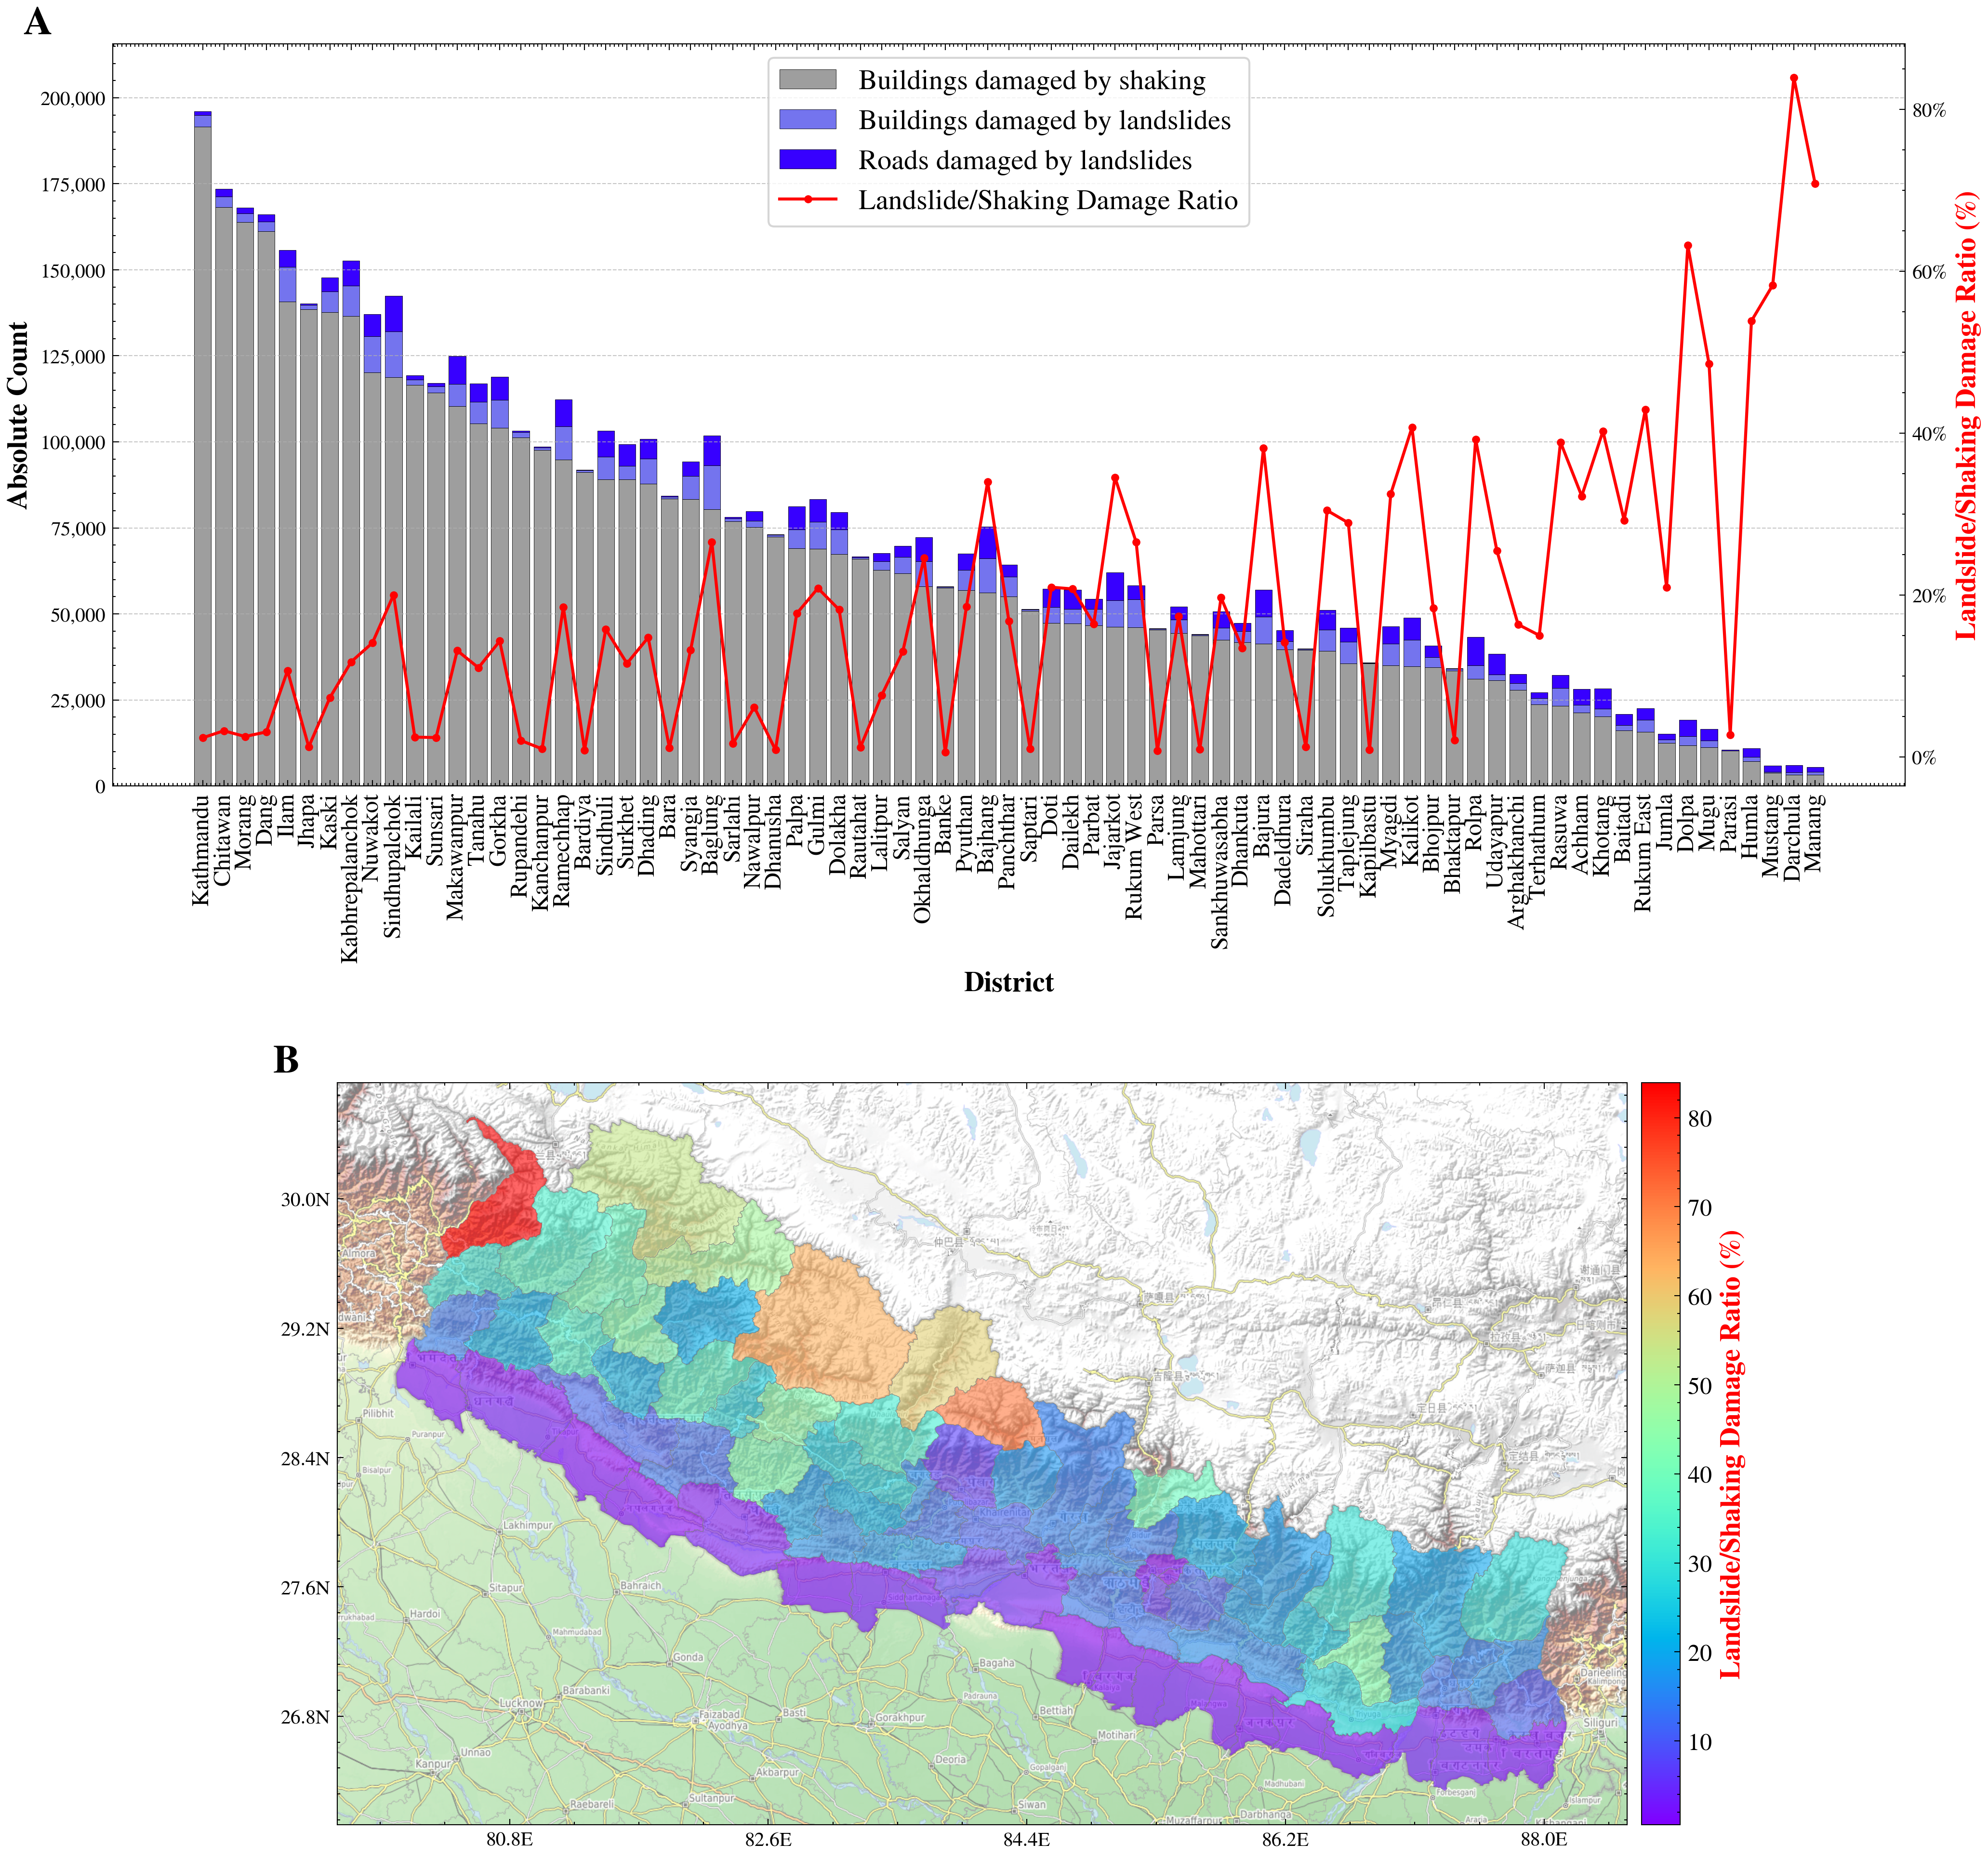
\includegraphics[width=1\linewidth]{./FIGURES/Fig3_district_impacts_ratio.png}
    \caption{A, district-wise plot of the range of buildings damaged by earthquake shaking (grey), buildings damaged by landslides (light blue), and road segments damaged by landslides (medium blue) across the 30 scenario earthquakes. The minimum values for all three types of impact are 0 in each district, so the height of each bar segment shows the range in possible outcomes across the 30 scenarios. Total bar height shows the worst-case number of impacts from both shaking and landsliding in each district. Bars are ordered by the highest maximum number of shaking-damaged buildings. The red line (right-hand axis) shows worst-case landslide impacts on buildings and roads as a percentage of the worst-case number of buildings damaged by shaking. B, district-wide map of worst-case landslide impacts on buildings and roads as a percentage of the worst-case number of buildings damaged by shaking. Note that the highest values are found in sparsely-populated mountain districts in northern Nepal.}
    \label{fig:district_ratio}
\end{figure}

Exceedance plots by district show that between 33\% and 63\% of scenarios result in at least one completely damaged building per district (Figure~\ref{fig:district_exceedance}A). In comparison, 30\% to 87\% of scenarios cause at least one building damaged by landslides (Figure~\ref{fig:district_exceedance}B), and 30\% to 77\% result in at least one road segment damaged by landslides (Figure~\ref{fig:district_exceedance}C). However, the median number of landslide-induced impacts is generally below 10 per district, confirming that landslide impacts are less frequent than shaking impacts but still widespread across scenarios. As expected, the exceedance probability patterns show distinct physiographic variations \citep{upreti_physiography_2001}. Districts in the southern Terai lowlands have high exceedance probabilities for shaking damage but consistently low probabilities for landslide impacts, reflecting their large building exposure but limited slope instability. In contrast, hill region districts have more variable exceedance patterns, with several districts showing higher landslide exceedance probabilities than shaking probabilities, particularly for road damage. High mountain districts have the most variable patterns, with some showing very low exceedance probabilities due to sparse infrastructure, while others have disproportionately high landslide exceedance probabilities relative to their larger shaking exposure. These physiographic trends highlight how topographic setting fundamentally controls the relative importance of different hazard components across Nepal's diverse landscapes.

\begin{figure}[H]
    \centering
    \includegraphics[width=1\linewidth]{./FIGURES/Fig4_district_exceedance_curves.png}
    \caption{A, exceedance probability of buildings damaged by earthquake shaking in each of the 77 districts in Nepal across the 30 scenario earthquakes. Each line shows an exceedance curve for a single district. Curves are coloured by physiographic setting of each district. Median impacts for each district across the ensemble are shown by where the curves intersect the 50\% line (dashed horizontal line), while worst-case impacts are shown by the intersection with the x axis. B, exceedance probability of buildings damaged by landslides in each district. C, exceedance probability of road segments damaged by landslides in each district.}
    \label{fig:district_exceedance}
\end{figure}

District-level variability is further explored in Figure~\ref{fig:standard_deviation}, which maps the standard deviation of impacts for each district. In absolute terms, the standard deviation is highest for shaking-induced building damage (Figure~\ref{fig:standard_deviation}A), reflecting the large number of buildings exposed to shaking. However, the standard deviation for landslide-related impacts (Figure~\ref{fig:standard_deviation}B, C) reveals distinct hotspots in the Hill and Mountain districts. This indicates, as expected, that while shaking damage is widespread, severe landslide impacts are more scenario-dependent, occurring at high intensities only under specific earthquake conditions.

Importantly, building damage from shaking and building or road damage from landsliding have different spatial footprints across Nepal. Districts with the largest expected numbers of damaged buildings, both in the median and in the worst-case scenarios, are concentrated in the more populated southern and central areas of the country (Figure~\ref{fig:worst_case_maps}A), highlighting not only building density but also patterns of infrastructure vulnerability. Districts in the more remote and more sparsely-populated northeast have relatively low total numbers of shaking-damaged buildings, even in the worst case. In contrast, while the absolute numbers of expected landslide impacts are lower, the largest number of landslide impacts are concentrated in the hill and mountain districts across Nepal (Figure~\ref{fig:worst_case_maps}C, E). Road impacts from landslides are widely distributed through the hill and mountain districts, with particular hotspots in Sindhupalchok, Baglung, Rolpa, Bajura, and Bajhang districts (Figure~\ref{fig:worst_case_maps}E). These areas should be considered at the highest risk of disruption to the road network after a future large earthquake. Building impacts from landslides are more focused on the hill districts, likely because of the concentration of population in those areas (Figure~\ref{fig:worst_case_maps}C). Not surprisingly, expected landslide impacts are lower in the flat-lying southern districts of the Terai, along the border with India (Figure~\ref{fig:worst_case_maps}C, D). The dominance of shaking impacts over landslide impacts means that their sum, which we take as the worst-case expected total number of earthquake impacts, mirrors the distribution of shaking damage, although numbers of impacts are notably higher in the hill districts in particular (compare Figure~\ref{fig:worst_case_maps}C and A).

\begin{figure*}
    \centering
    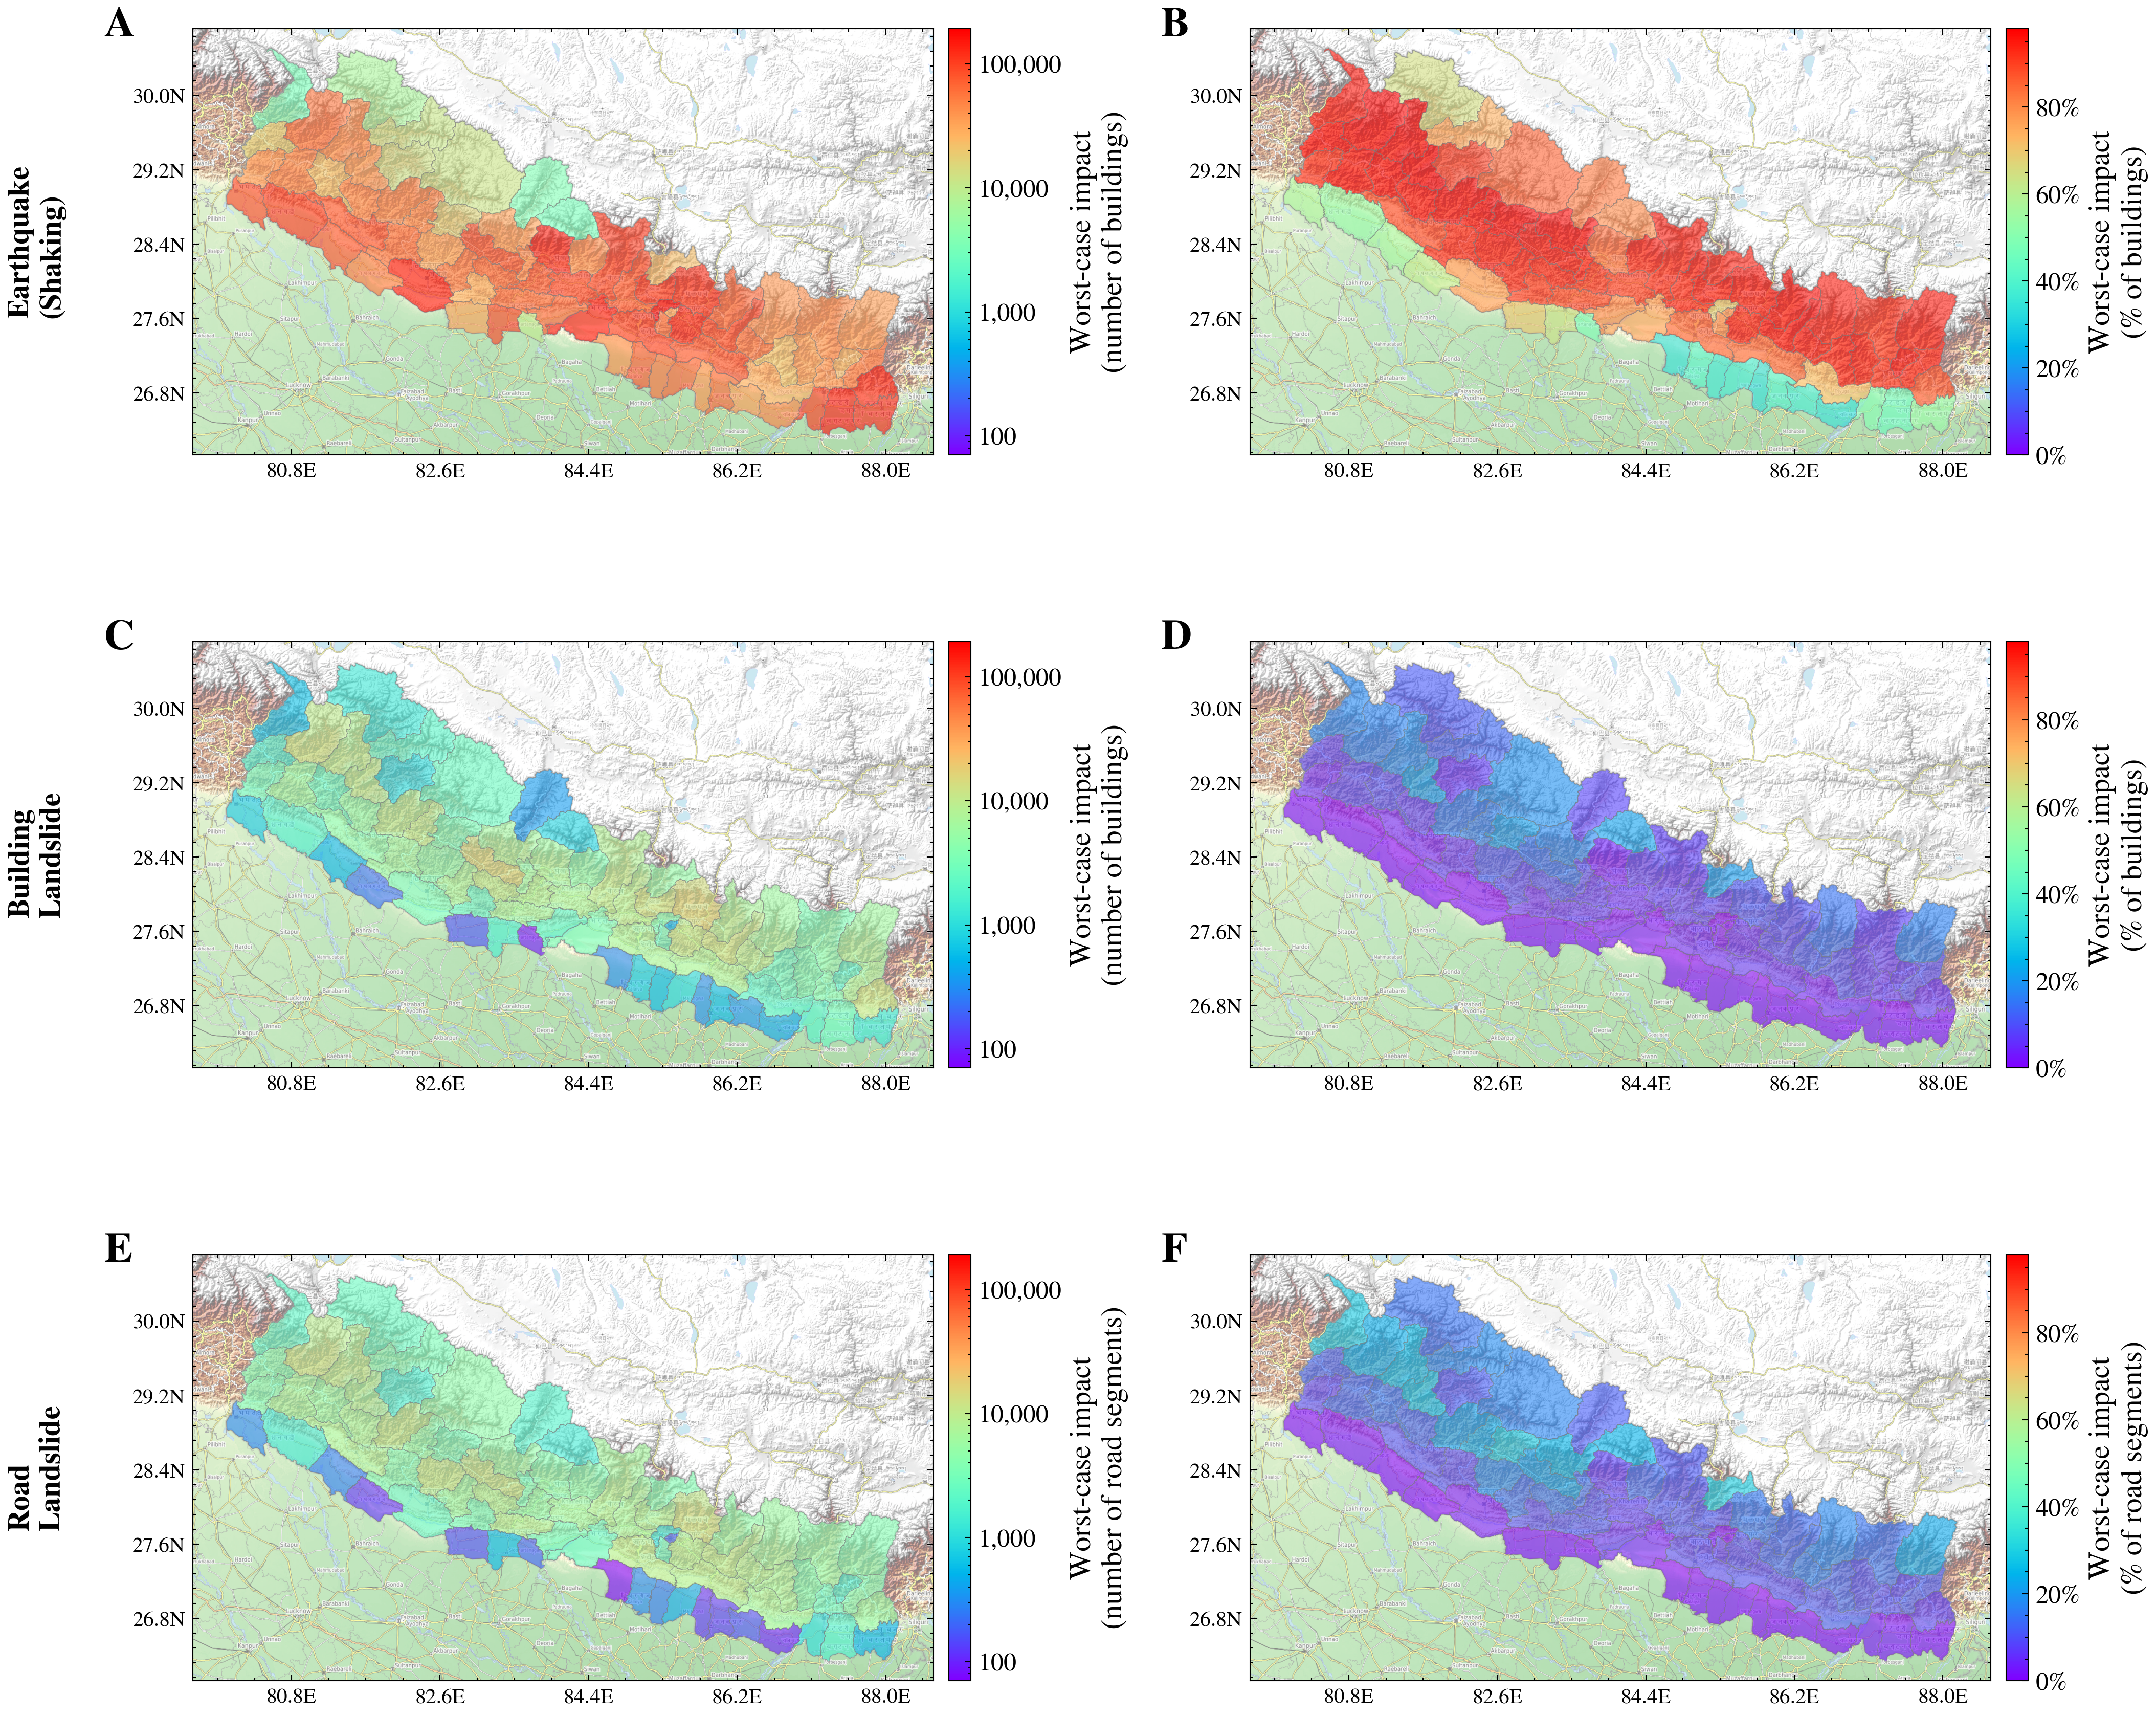
\includegraphics[width=1\textwidth]{./FIGURES/Fig5_worst_case_absolute_proportional.png}
    \caption{Maps of earthquake impacts by district. Left column: Worst-case absolute numbers of (A) buildings damaged by shaking, (C) buildings damaged by landslides, and (E) road segments damaged by landslides. Right column: Worst-case proportion (in percent) of (B) buildings damaged by shaking, (D) buildings damaged by landslides, and (F) road segments damaged by landslides.}
    \label{fig:worst_case_maps}
\end{figure*}

\begin{figure}
    \centering
    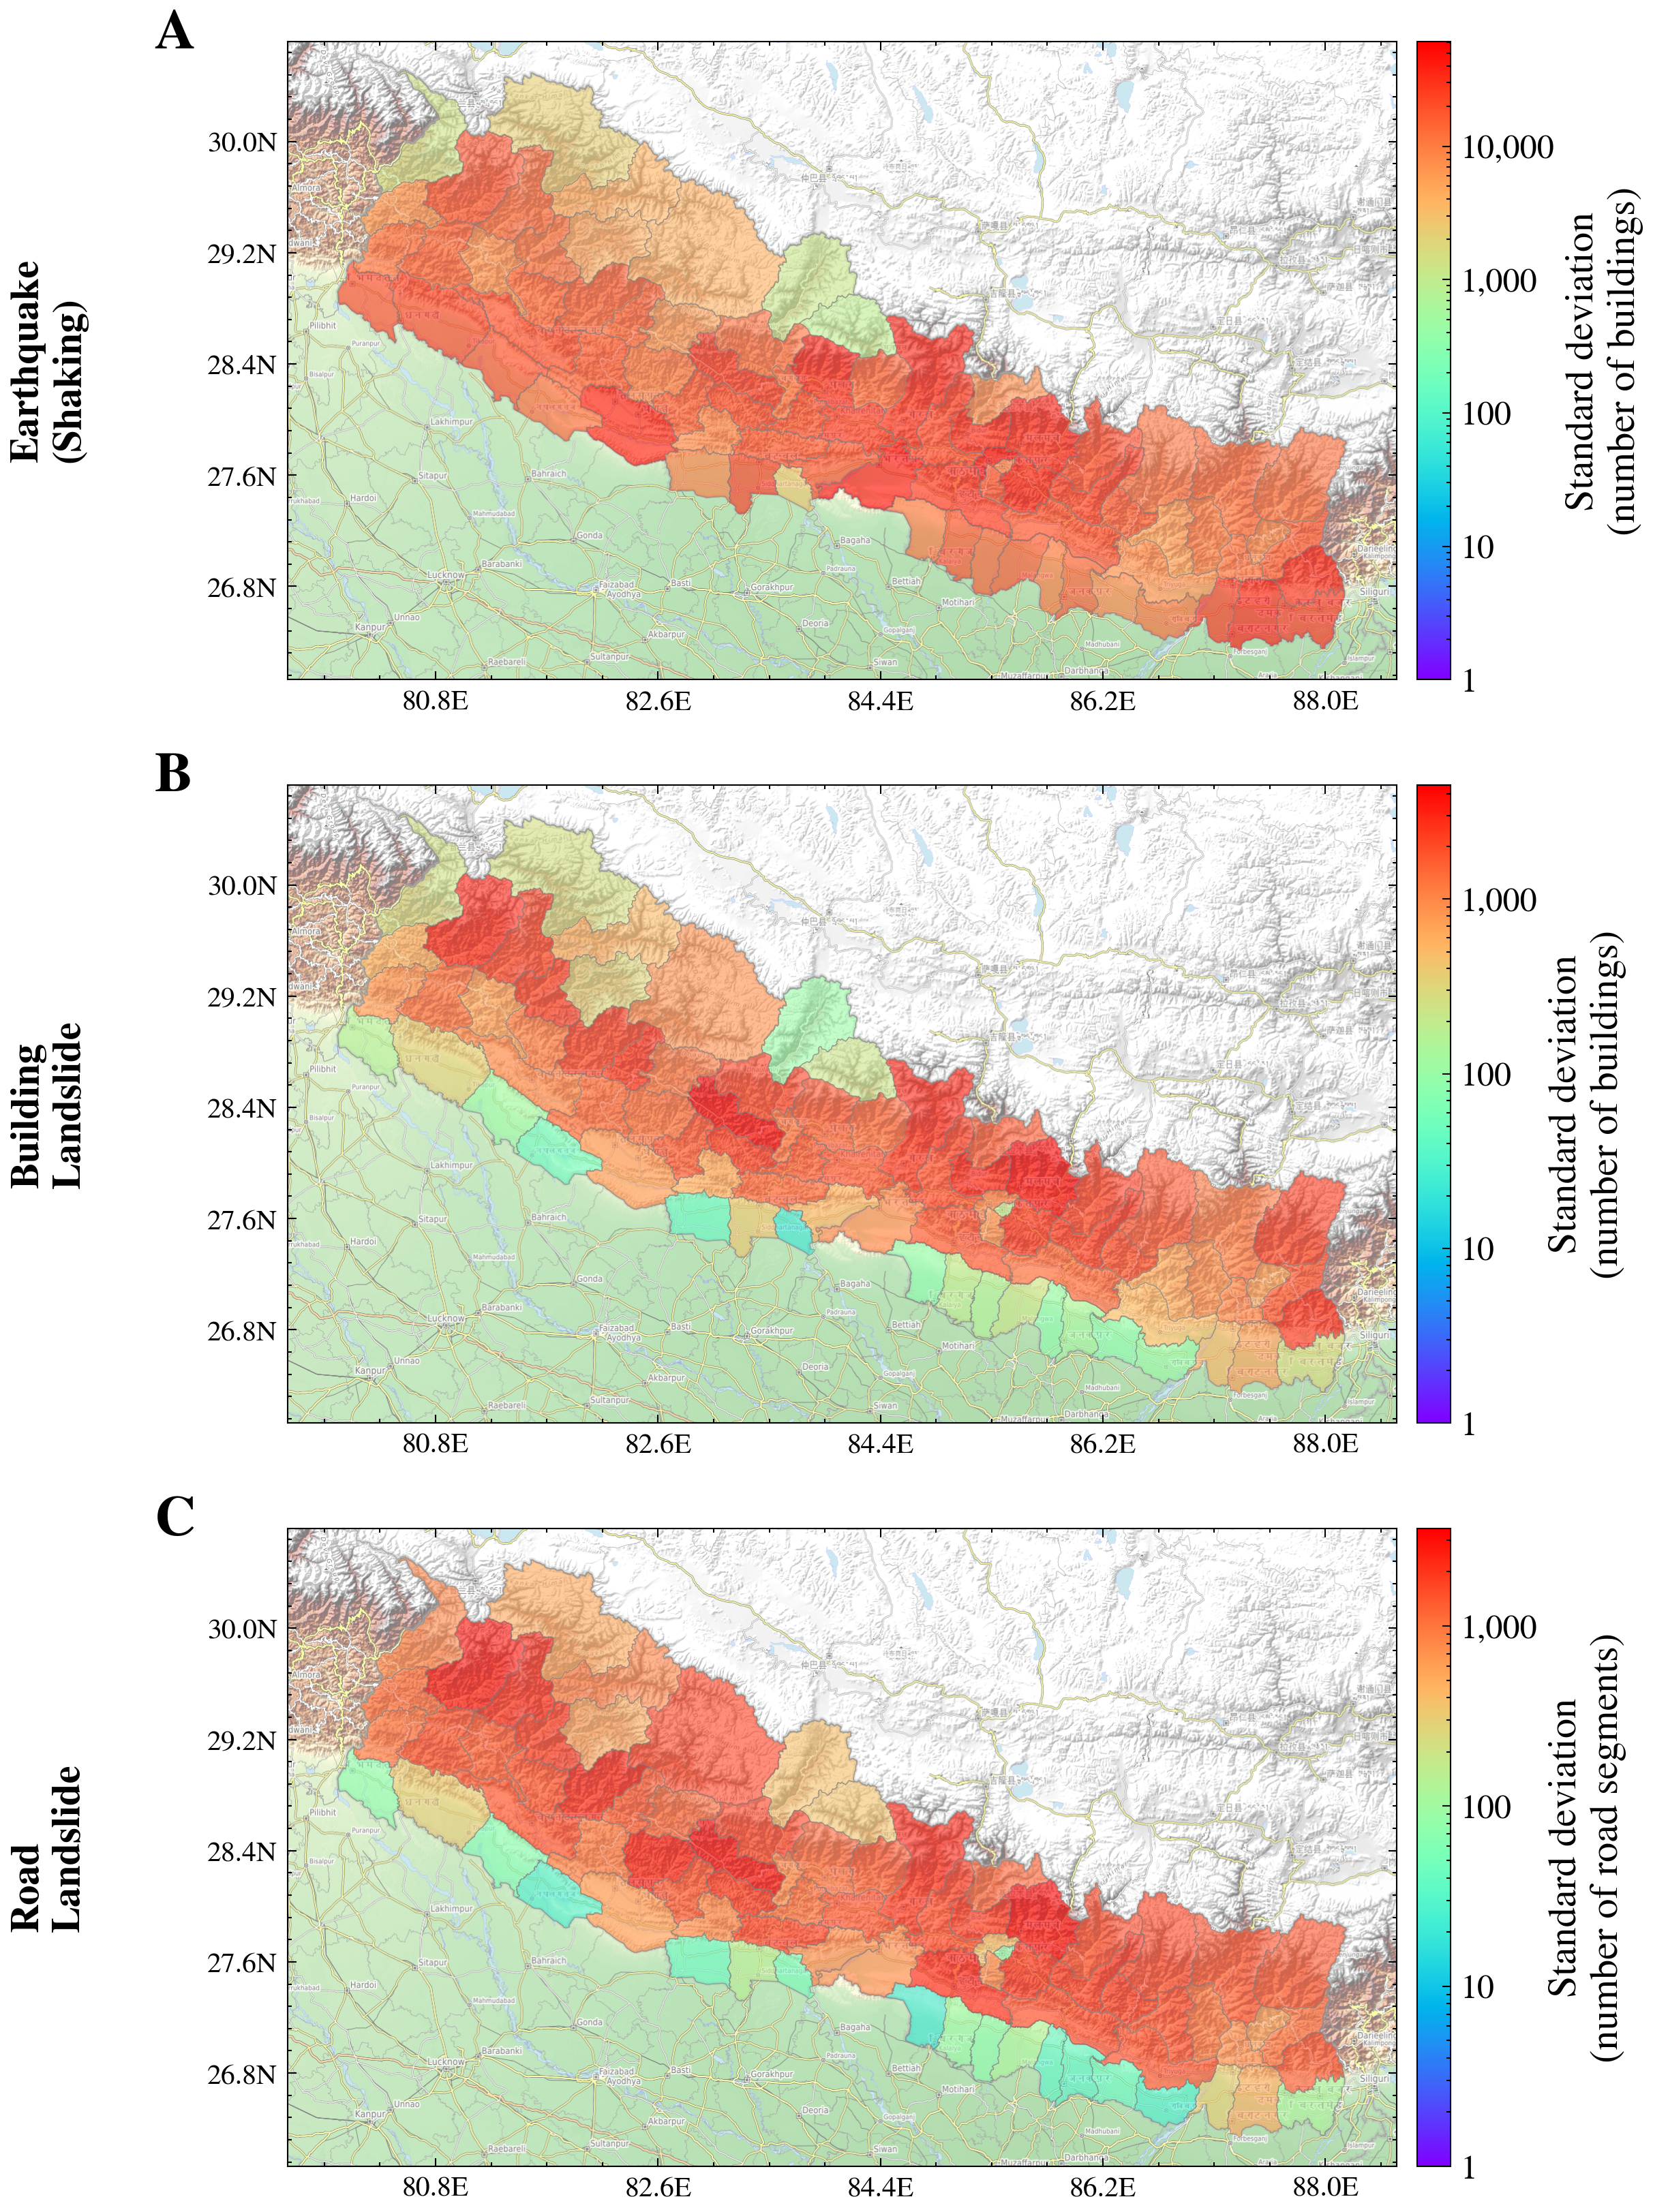
\includegraphics[width=0.75\linewidth]{FIGURES/Fig6_standard_deviation.png}
    \caption{Standard deviation of (A) buildings damaged by shaking, (B) buildings damaged by landslides, and (C) road segments damaged by landslides. Note the different scales between panels.}
    \label{fig:standard_deviation}
\end{figure}

\subsection{Vulnerability and accessibility}

The index of remoteness from health facilities (Figure~\ref{fig:remoteness}A) shows values ranging from near 0 in southern districts to over 0.8 in northern regions, with the highest values observed in the northwestern districts of Dolpa, Bajhang, Darchula, Humla and Bajura. The scatter plot comparing the district headquarters remoteness index against the health posts remoteness index (Figure~\ref{fig:remoteness}B) shows most districts positioned below the 1:1 line. This indicates that remoteness values from district headquarters are typically higher than those from health posts for the same districts. Identified outliers include Bajhang and Darchula, with the district of Manang being the outlier above the 1:1 line.

\subsection{Remoteness, impacts, and risk scores}

The relationship between remoteness and road network vulnerability is further detailed in Figure~\ref{fig:remoteness} (bottom panels). Figure~\ref{fig:remoteness}C demonstrates that districts categorized as having 'High' remoteness experience a significantly larger proportion of road network damage (median $\approx 24\%$) compared to 'Low' remoteness districts (median $\approx 9\%$). Conversely, Figure~\ref{fig:remoteness}D shows that in terms of absolute numbers, the 'Low' remoteness districts (often more urbanized) bear the highest total impact count (shaking and landslides combined), yet the 'High' remoteness areas face disproportionate functional disruption relative to their existing infrastructure.

\begin{figure}[H]
    \centering
    \includegraphics[width=1\linewidth]{./FIGURES/Fig7_remoteness_analysis.png}
    \caption{Combined analysis of remoteness and vulnerability. 
    A, Map of Remoteness Index regarding access to Health Posts. 
    B, Comparison of District Headquarters vs. Health Posts remoteness indices (dashed line represents 1:1 relationship). 
    C, Box plots showing the percentage of road network damaged by landslides across remoteness categories (Low, Medium, High). 
    D, Box plots showing total worst-case impact (buildings and roads, log scale) across remoteness categories. 
    Note that highly remote districts face higher proportional road damage (C) despite lower absolute impact counts (D).}
    \label{fig:remoteness}
\end{figure}

\begin{figure}[H]
    \centering
    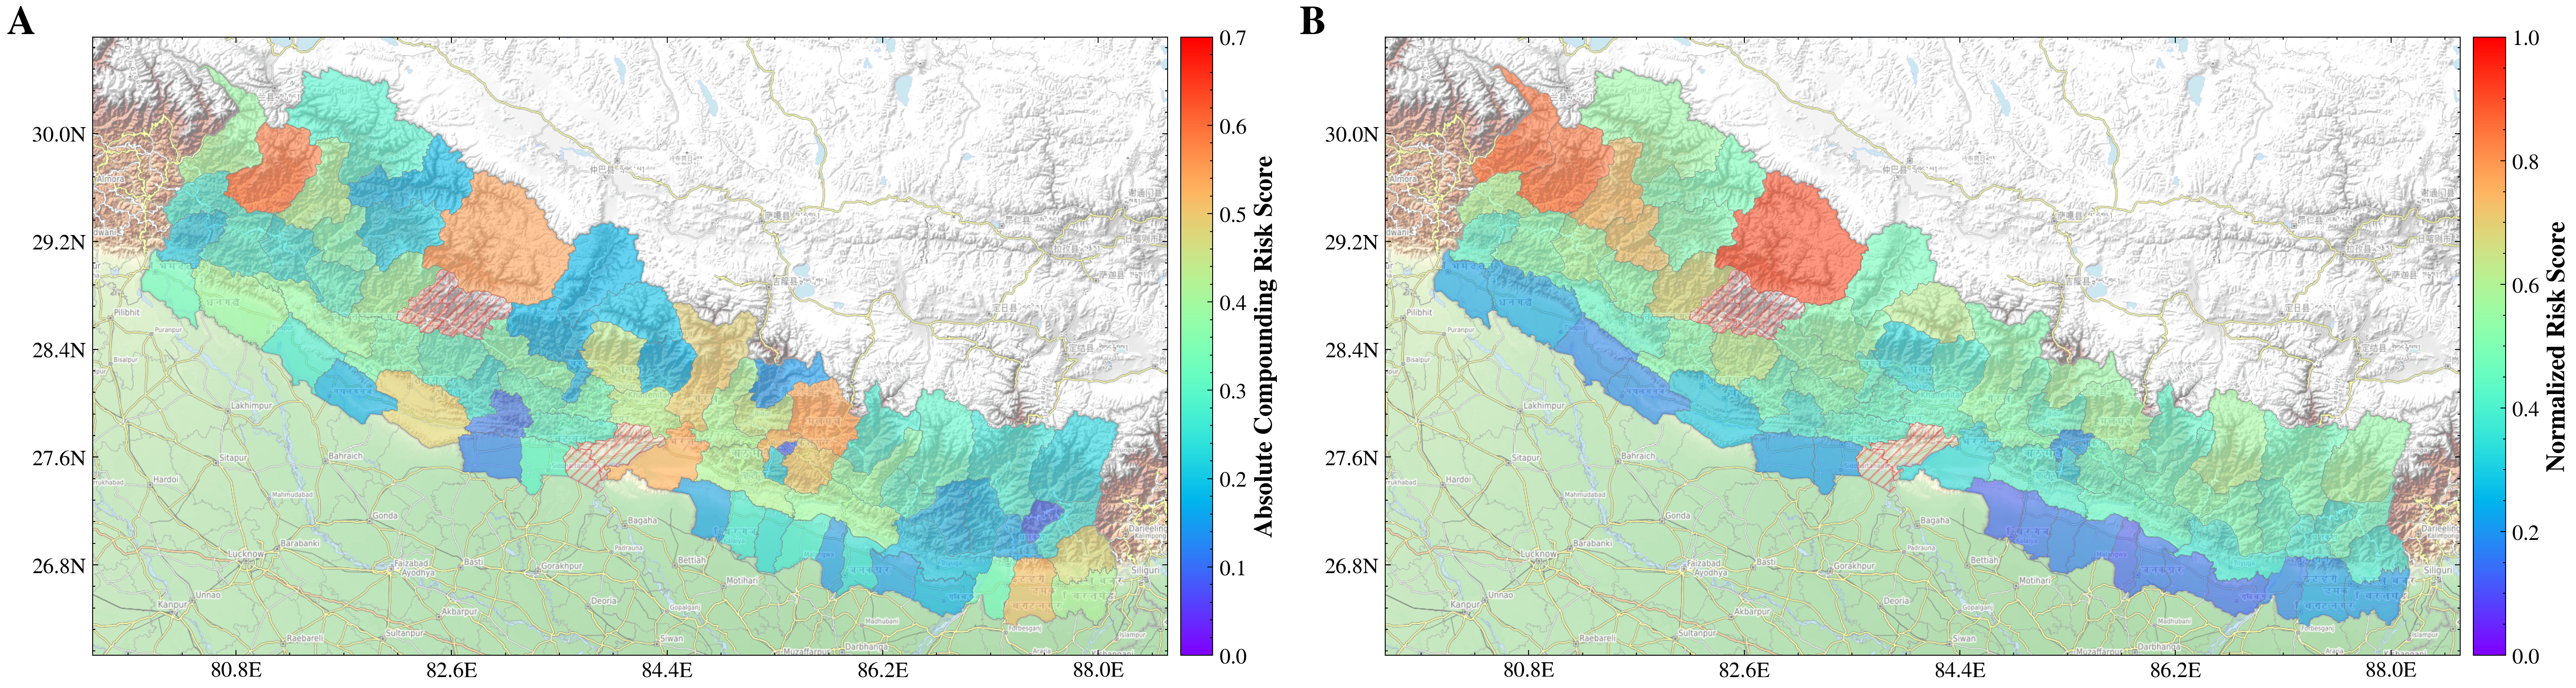
\includegraphics[width=1\linewidth]{./FIGURES/Fig8_risk_scores.png}
    \caption{Maps of Multi-Hazard Risk Scores: (A) Absolute Compounding Risk Score identifying hotspots of large-scale compounding disaster; (B) Normalized Risk Score identifying districts where the community is most severely threatened regardless of size.}
    \label{fig:risk_score}
\end{figure}

\section{Discussion}

\subsection{Differences between shaking-only and multi-hazard scenario outcomes}

Robinson et al. \citep{Robinson2018} emphasized shaking-induced impacts concentrated near rupture zones, providing valuable insights through scenario ensemble approaches. Building on this previous work, our study incorporates landslides as cascading hazards to expand the analysis. Overall, the correlation between the previous work align well at district level with a correlation of 0.78 which is expected as the earthquake ensemble members are similar and represent a large part of the multi-hazard damage. The multi-hazard scenarios reveal broader spatial impacts beyond zones affected by shaking, especially in steep, landslide-prone areas. This expanded footprint is evident when comparing the distribution of shaking damage with landslide-related damage. Figure~\ref{fig:district_exceedance} shows that districts in the High Mountain and Hill physiographic regions experience higher exceedance probabilities of landslide impacts than shaking impacts alone.

Substantial variation was also observed in the proportion of damage caused by shaking versus landslides (Figure~\ref{fig:district_ratio}). Some districts that appeared moderately affected in shaking-only scenarios showed higher overall impacts when landslides were included. Figure~\ref{fig:standard_deviation} shows higher standard deviation for landslide damage in several northern districts compared to shaking, indicating that significant impacts occurred only under certain scenarios. These variations point to the need for localized risk management strategies that consider both seismic and landslide hazards.

\subsection{Road network impacts and compounding effects of remoteness}

The scenario ensemble also quantified impacts on road networks. Figure~\ref{fig:worst_case_maps} (E, F) shows that road damage from landslides was widespread, affecting multiple districts. A correlation was observed between road damage and district remoteness (Figure~\ref{fig:remoteness}). Districts with higher remoteness scores consistently experienced a larger share of road damage. Districts such as Dolpa, Bajhang, and Darchula face overlapping risks from remoteness and road exposure, reducing access and increasing vulnerability.

\subsection{Scale dependence of hazards}
WIP

\subsection{Limitations}

Several limitations are inherent to the ensemble approach. While the analysis captures large-scale impacts from high-magnitude earthquakes, it does not include locally destructive moderate-magnitude events such as the 2023 Jajarkot earthquake (Mw 5--6). These events can cause severe localized impacts and warrant dedicated modelling. Additionally, we focus here on physical infrastructure damage and do not explicitly model fatalities, as infrastructure impact alone is not sufficient for risk-to-life estimates from landslides \citep{VanWykDeVries2024}. Future work integrating dynamic exposure and mobility is expected to improve casualty estimation.

\subsection{Urban--rural risk contrast and geographic disparities}

The analysis highlights differences in hazard and risk profiles between urban and rural areas. Urban districts, with denser infrastructure and better accessibility, showed higher proportions of shaking-related damage. In contrast, remote rural mountainous districts experience greater exposure to landslide-related impacts and limited access to critical services, complicating emergency response. This contrast aligns with broader discussions on geographic determinism \citep{Diamond1997}. Nepal's topographic diversity certainly contributes to uneven disaster preparedness and recovery capacities between regions, emphasizing the importance of place-based approaches to risk reduction.

\section{Conclusions}

This study extends ensemble-based earthquake risk assessments by incorporating landslide hazards into the scenario framework developed by Robinson et al. \citep{Robinson2018} by leveraging the hyperedge method for cascading scenario generation developed by Dunant et al. \citep{Dunant2025}. The multi-hazard ensemble reveals that landslides substantially increase the spatial extent of risk, particularly in steep and remote regions of Nepal. Although landslides account for a smaller proportion of total building damage compared to shaking, their contribution to overall risk is substantial. In several districts, the ratio of worst-case landslide to shaking impacts exceeds 50\%, indicating that landslide damage may dominate under specific scenarios. This underscores the spatial heterogeneity in hazard impacts across the country.

The analysis also shows that landslides significantly affect transport infrastructure, particularly in remote areas, thereby reducing access to healthcare facilities and complicating emergency response. The observed correlation between remoteness and road damage highlights the importance of pre-event planning and infrastructure resilience, as emphasized in national frameworks such as the Earthquake Response Preparedness Plan (ERPP). The current ensemble does not account for moderate-magnitude (M5-6) but locally destructive events, such as the 2023 Jajarkot earthquake. This points to the need for complementary localized modelling approaches to capture risk in underrepresented areas.

Finally, the findings reflect a persistent urban--rural risk divide, shaped by geographic and infrastructural disparities. Addressing this divide remains a key priority for disaster risk reduction. Future improvements in fatality modelling and the integration of high-resolution mobility and exposure data will be essential for producing more accurate and actionable multi-hazard risk assessments.

\section*{Acknowledgments}
This research was supported by a grant from the UKRI Global Challenges Research Fund Multi-Hazard and Systemic Risk programme (NE/T01038X/1). The AW3D DEM is licensed via Durham University (UK), with funding from the DFID-UKRI SHEAR programme (project number: 201844-112) (AW3D 5 m DEM \textcopyright JAXA, RESTEC and NTTDATA).

\section*{Author Contributions}
ALD, TRR, NJR, and others secured the funding for the research reported here. The study was conceived by AD, TRR, ALD, and NJR. AD developed the numerical model with input from TRR, ALD, NJR, RMR, and MK. AD ran the numerical experiments with assistance from TRR and RMR. AD, ALD, and TRR wrote the original draft of the manuscript. All authors contributed to analysis of the results and review and editing of the manuscript.

% -------------------- REFERENCES --------------------
% The following command will include references from references.bib
\bibliography{references}

% -------------------- SUPPLEMENT --------------------
\clearpage
\appendix
\renewcommand{\thefigure}{S\arabic{figure}}
\setcounter{figure}{0}

\section*{Supplemental Information}

\begin{figure}[H]
    \centering
    \includegraphics[width=1\linewidth]{./FIGURES/FigS1_fragility_functions.png}
    \caption{Fragility functions used in the hypergraph network modelling, modified from Dunant et al. (2025). Each panel shows the functions for a different building type in the METEOR dataset, relating peak ground acceleration (PGA, in g) to the probability of a complete damage state. Note that each fragility function is defined by two parameters: a scale parameter that sets the PGA value for a 50\% probability of complete damage, and a standard deviation (std) that defines the spread of the curve. Parameter values and sources for the fragility curves are included in the plots and in the references.}
    \label{fig:S1}
\end{figure}

\begin{figure}[H]
    \centering
    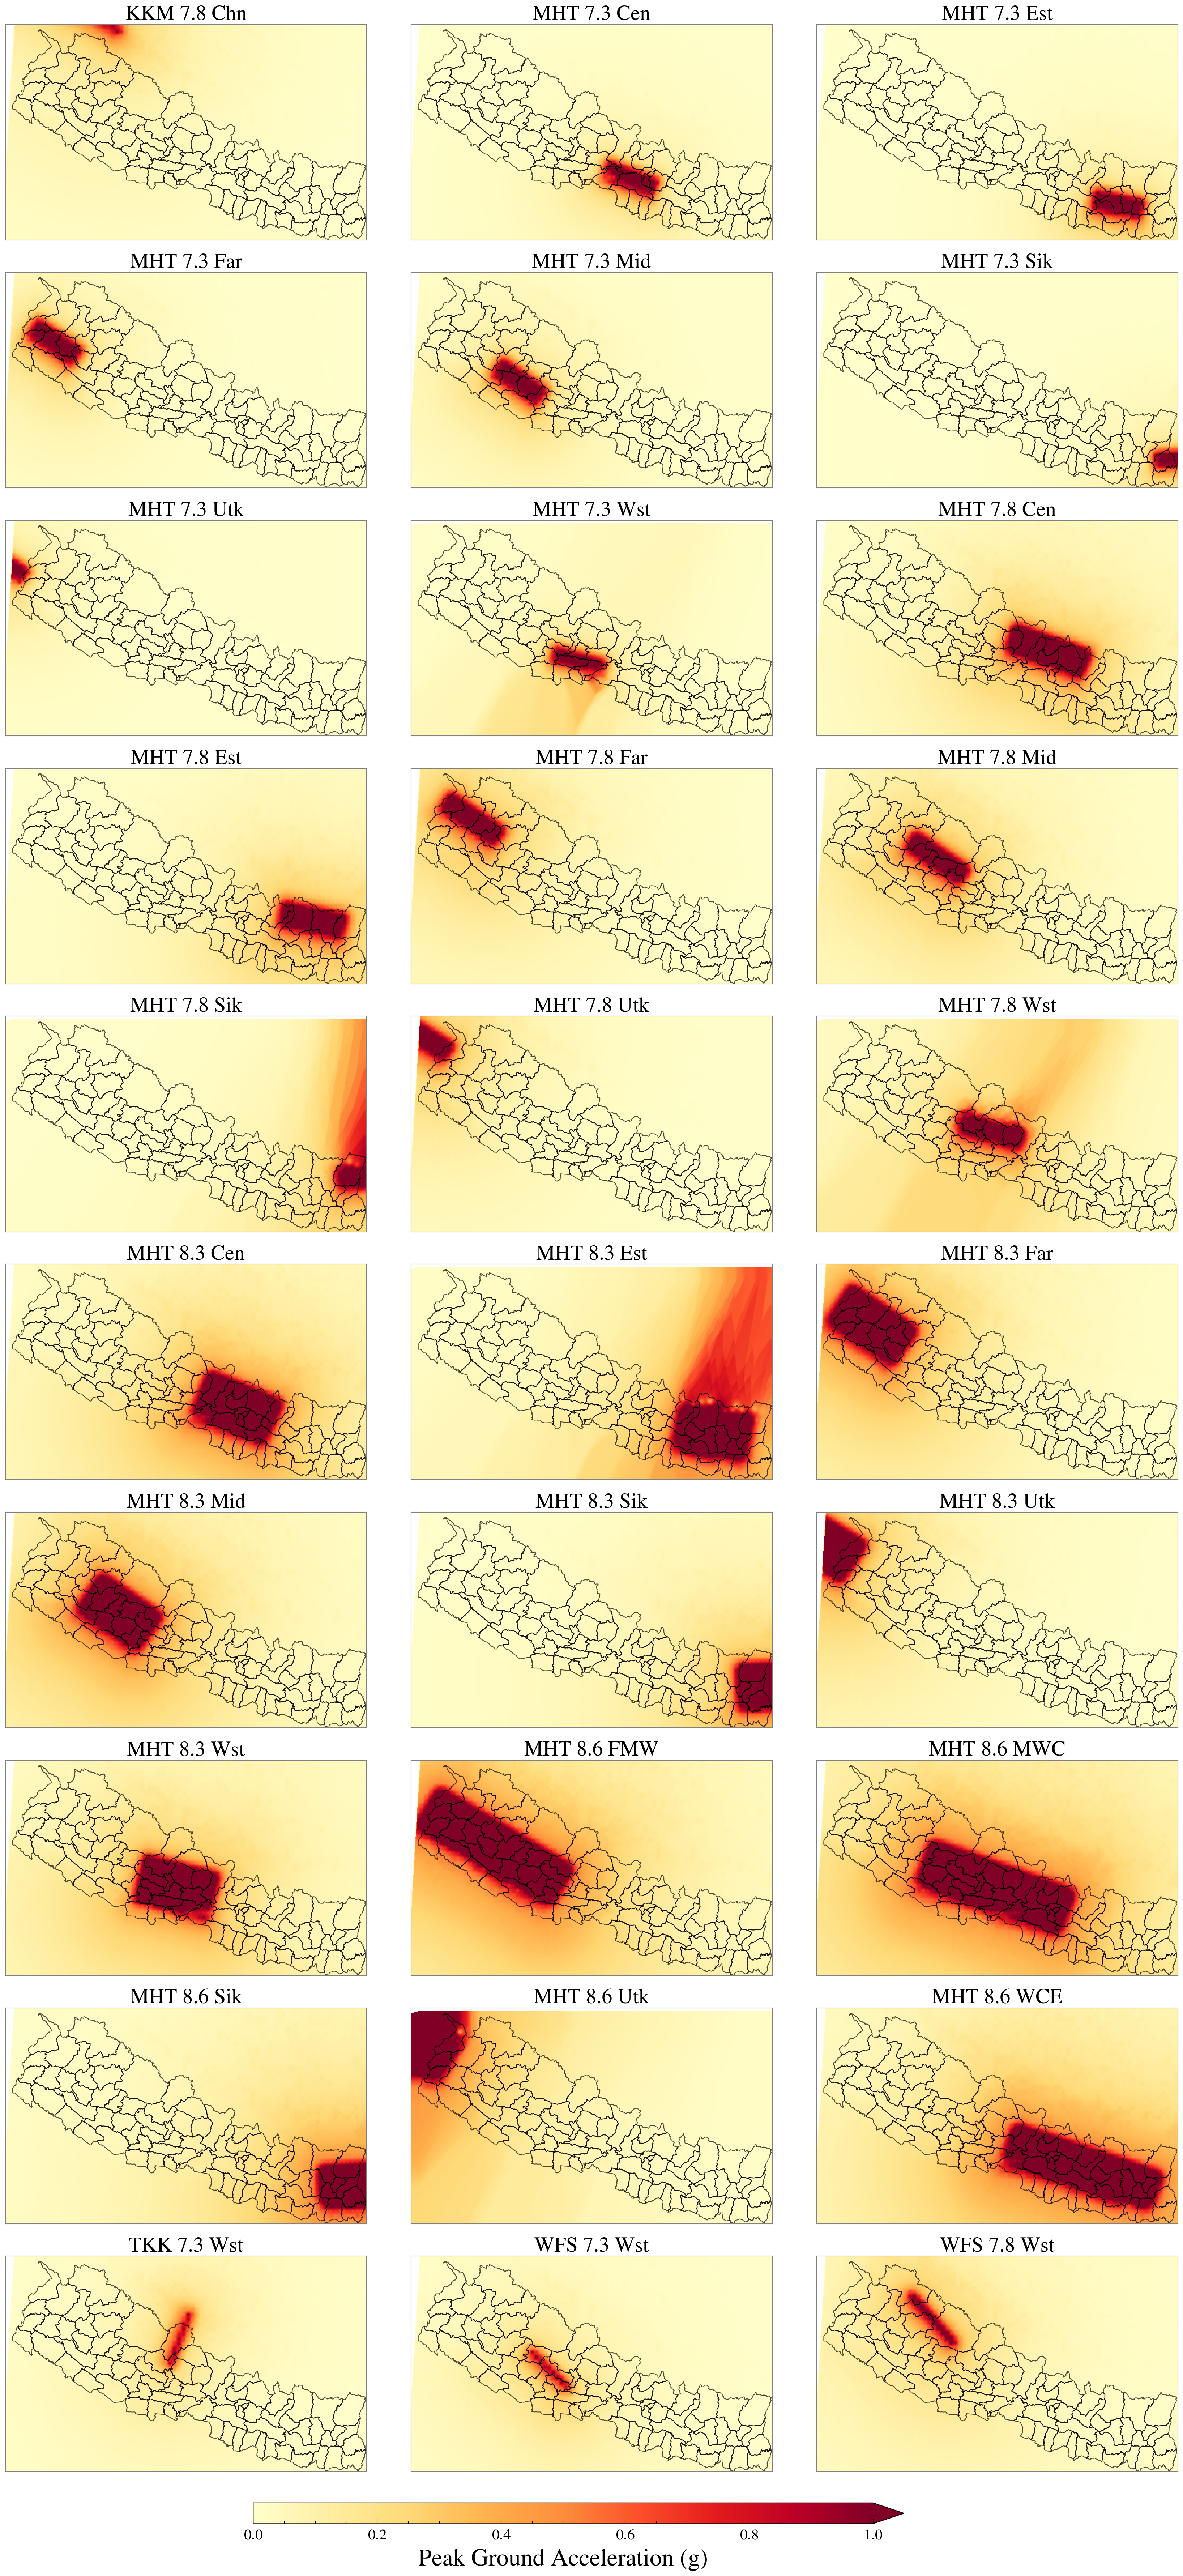
\includegraphics[width=0.75\linewidth, height=17cm]{./FIGURES/FigS2_pga_ensemble_maps.png}
    \caption{Maps of peak ground acceleration (PGA, in g) for each of the 30 scenario earthquakes in the ensemble.}
    \label{fig:S2}
\end{figure}

\begin{figure}[H]
    \centering
    \includegraphics[width=0.75\linewidth, height=17cm]{./FIGURES/FigS3_median_collapse_probability.png}
    \caption{Maps of the median probability of collapse for each of the 30 scenarios of the earthquake ensemble.}
    \label{fig:S3}
\end{figure}

\begin{figure}[H]
    \centering
    \includegraphics[width=1.0\linewidth]{./FIGURES/FigS4_remoteness_clusters.png}
    \caption{Determination of the number of remoteness clusters based on KMeans analysis and silhouette score.}
    \label{fig:S4}
\end{figure}

\begin{figure}[H]
    \centering
    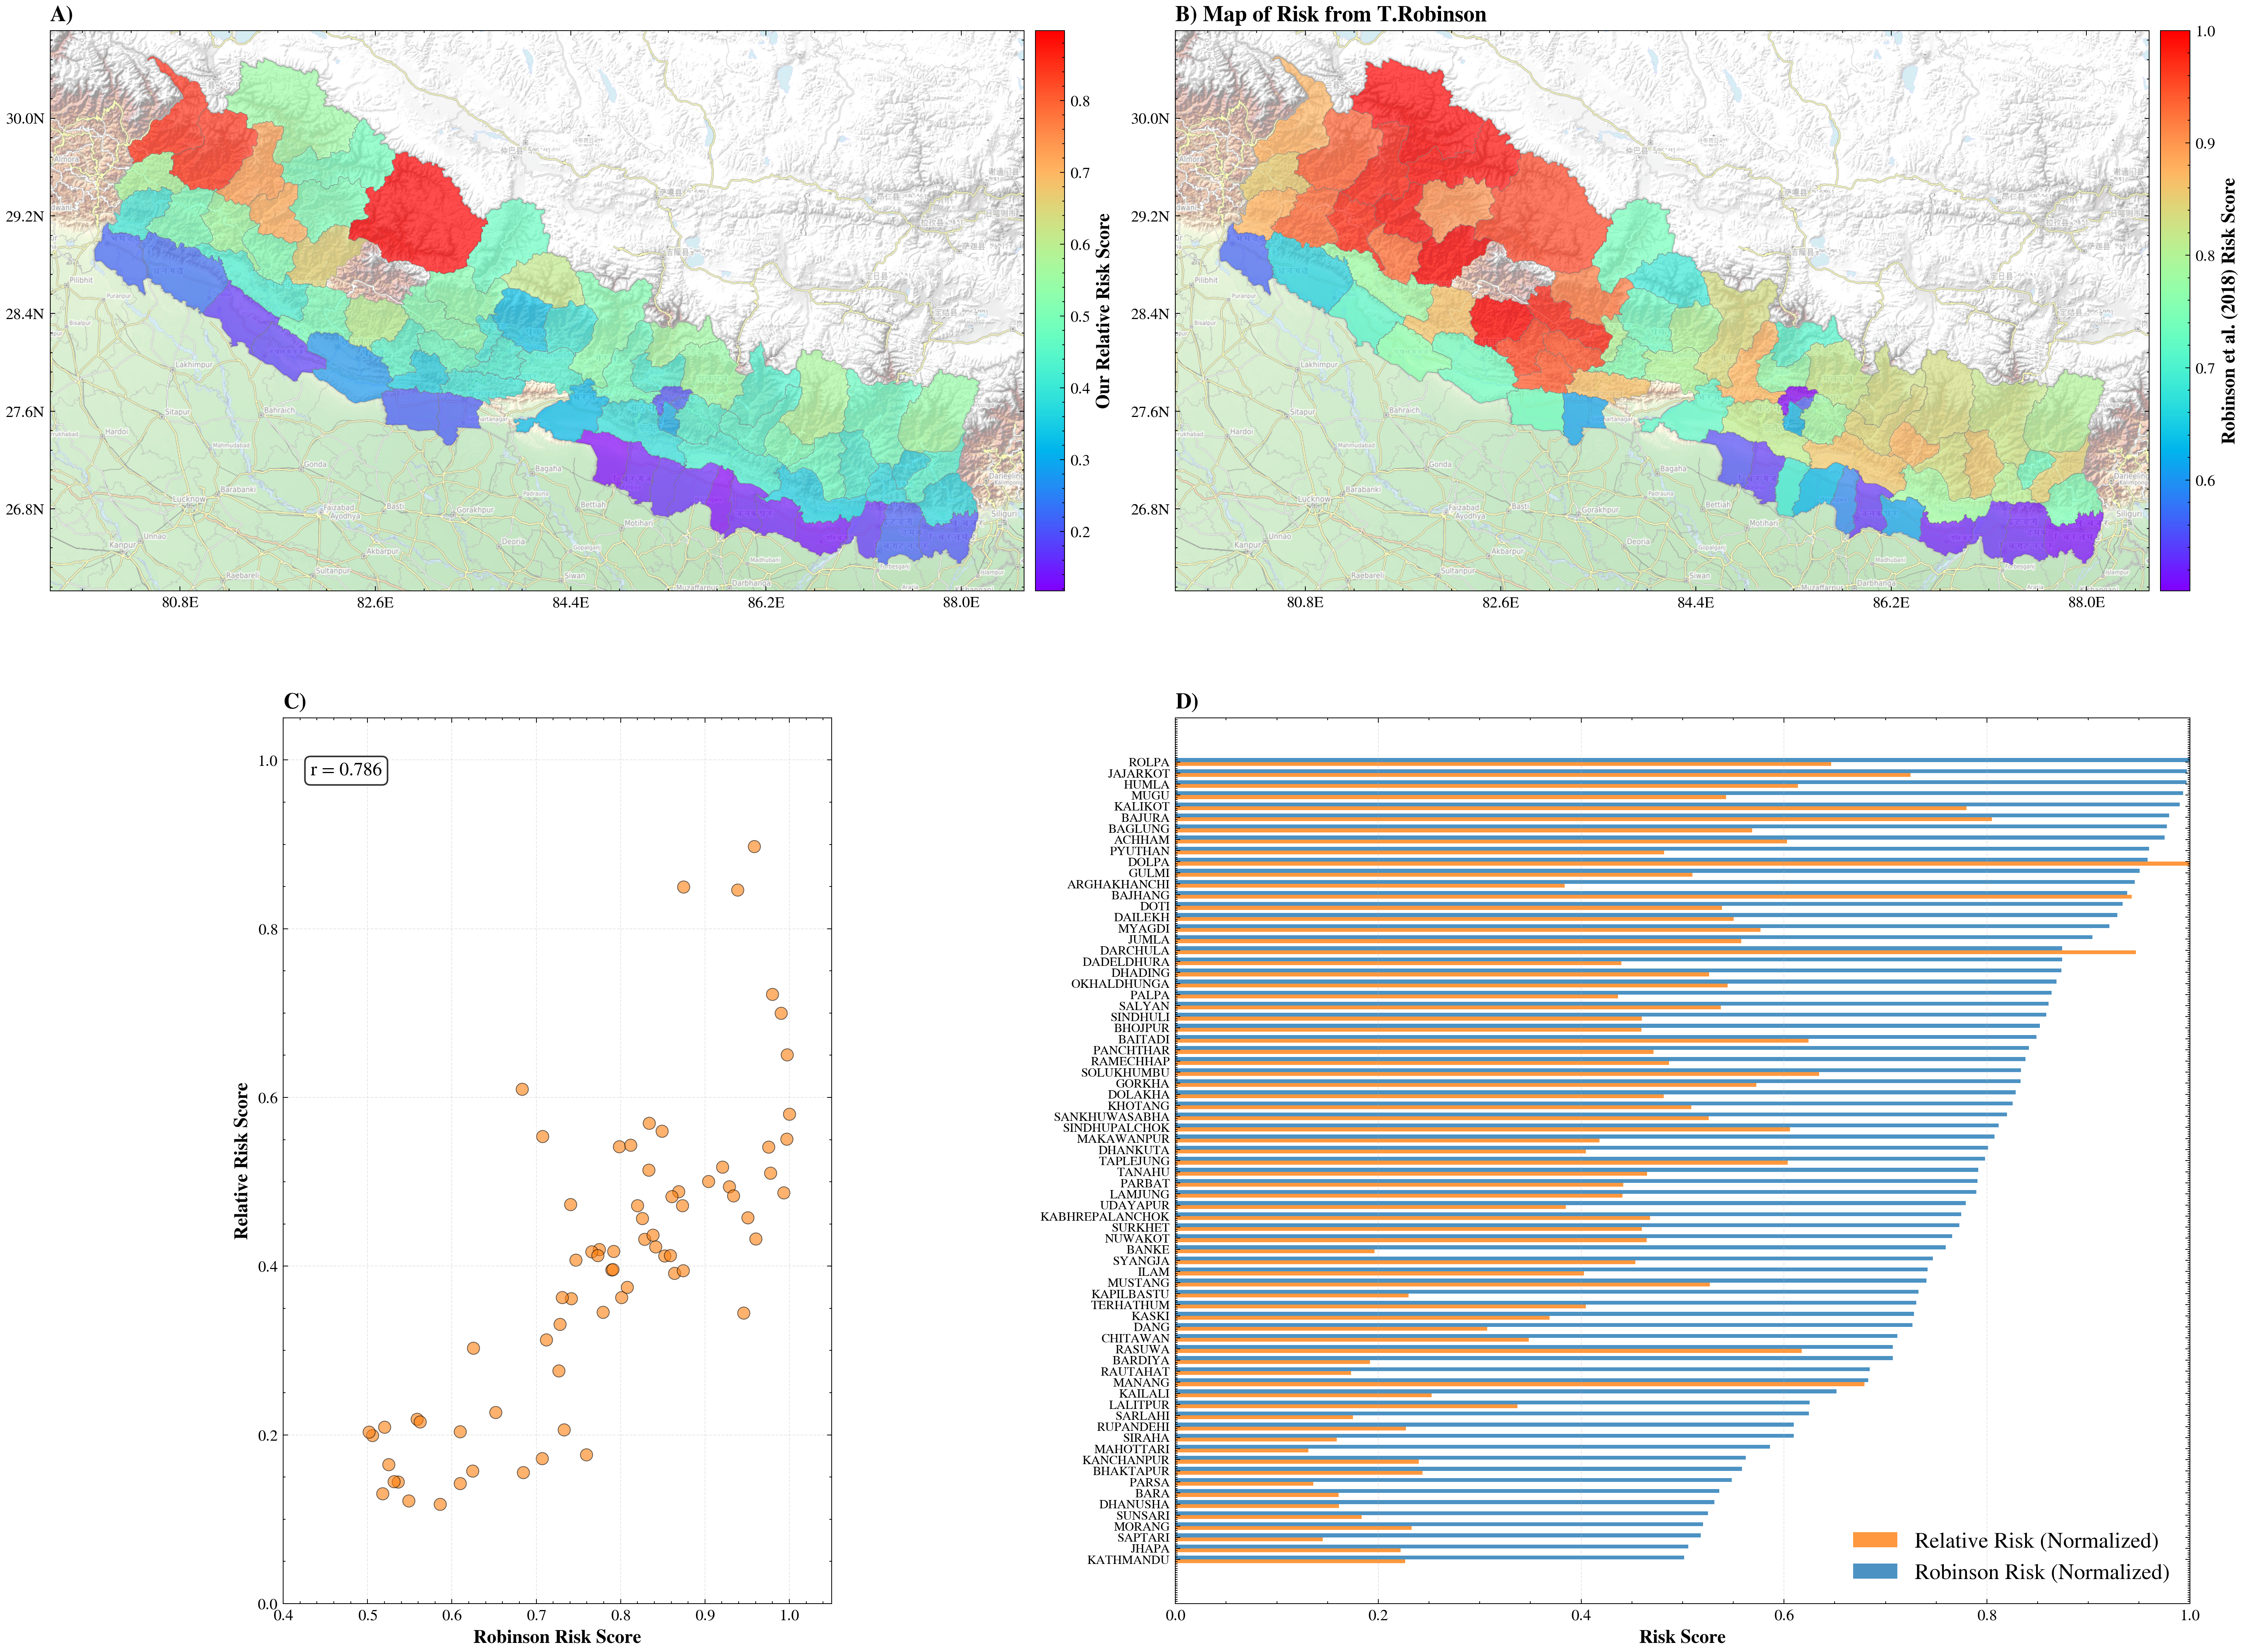
\includegraphics[width=1.0\linewidth]{./FIGURES/FigS5_robinson_comparison.png}
    \caption{Comparison of Normalized Risk Scores with Robinson et al. (2018) risk scores. (A) Horizontal bar plot showing the top 20 districts ranked by Robinson Risk Score, with side-by-side comparison of both scoring methods. (B) Scatter plot showing the correlation between Normalized Risk Score and Robinson Risk Score, with linear regression fit line (red) and 1:1 reference line (black dashed). The analysis includes 63 districts with complete data from both studies.}
    \label{fig:S5}
\end{figure}

\end{document}